\documentclass[journal]{IEEEtran}

% -------------------- Packages --------------------
\usepackage{graphicx}
\usepackage{cite}
\usepackage{amsmath}
\usepackage{amssymb}
\usepackage{booktabs}
\usepackage{multirow}
\usepackage{url}
\usepackage{xcolor} 
\usepackage{cuted} % Required to make the abstract full-width

% Define a lighter, standard hyperlink blue
\definecolor{hyperblue}{rgb}{0.0, 0.4, 0.8}

\usepackage{hyperref}
\hypersetup{
    colorlinks=true,
    linkcolor=hyperblue,
    filecolor=magenta,      
    urlcolor=hyperblue,
    citecolor=hyperblue,
    breaklinks=true 
}
% -------------------- Hyphenation --------------------
\hyphenation{op-tical net-works semi-conduc-tor}

\begin{document}

% =====================================================
% Title
% =====================================================

\title{SAARTHI: An AI-Powered Industrial Safety Copilot for Real-Time Excavator Hazard Detection}

% =====================================================
% Authors
% =====================================================

\author{
Sounak~Chowdhury,
Noel~Binu,
Member~3,
Member~4,
Member~5
}

\maketitle

% =====================================================
% Abstract & Keywords (Full Width)
% =====================================================

\begin{strip}
\vspace{-1.2cm} % Pulls the abstract up closer to the authors

\noindent\textbf{\textit{Abstract}---Keeping heavy machinery operators safe is difficult because most collision and fatigue monitors work in total isolation. A cabin camera doesn't know what is in the vehicle's blind spot, and proximity sensors cannot tell if a driver is falling asleep. Because these older systems rely on fixed, hard-coded rules, they generate constant false alarms on busy worksites. Eventually, operators just stop paying attention to them altogether. We built SAARTHI to solve this disconnect. It is a personalized AI copilot that fuses different safety feeds into a single Hybrid Decision Engine. The system actively combines spatial hazard tracking via YOLO, physiological data from MediaPipe, and raw machine telemetry. To evaluate the actual danger of a situation, an XGBoost-driven Contextual Risk Engine adjusts the baseline score based on weather, shift timing, and operator experience. Instead of relying on a static siren, intervention decisions are handled by a Proximal Policy Optimization (PPO) reinforcement learning model. The agent learns exactly when and how to alert the operator without causing alarm fatigue. We also built the interface to adapt automatically to the person in the seat, swapping standard audio for haptic feedback or high-contrast visuals based on their specific profile. Hosted on an asynchronous FastAPI backend, the architecture proves that multi-modal, highly personalized safety constraints can run in real time across industrial fleets without lagging.}

\vspace{0.3cm}

\noindent\textbf{\textit{Index Terms}---Industrial Safety, Computer Vision, YOLOv8, Excavator, Hazard Detection, Edge AI, Large Language Models.}

\vspace{0.6cm} % Adds breathing room before the Introduction starts
\end{strip}

% =====================================================
% Main Sections
% =====================================================

\section{Introduction}
\label{sec:introduction}

The construction and industrial manufacturing sectors are highly hazardous environments where rigorous safety monitoring is critical to preventing accidents. Workers constantly operate in close proximity to heavy machinery and dynamic spatial obstacles, making consistent and safe reactions to traffic and machinery hazards a major challenge. A significant, yet often overlooked, issue in modern safety monitoring is alarm fatigue; repeated exposure to static or continuous alarm patterns causes workers to become desensitized, thereby drastically reducing their vigilance and responsiveness to actual hazards over time \cite{lu2025reinforcement}. 

Operator impairment, specifically drowsiness, further compromises worksite safety. Drowsiness induced by sleep deprivation results in microsleeping and prolonged eyelid closures, both of which are critical early indicators of fatigue that lead to fatal misjudgments. Modern computer vision systems have proven highly effective at identifying these states by monitoring facial landmarks to compute the percentage of eyelid closure and estimating three-dimensional head poses \cite{owen2025drowsiness}. Concurrently, deep learning architectures like the You Only Look Once (YOLO) algorithm are widely utilized to rapidly and accurately detect external targets—such as workers and personal protective equipment—within complex, heavily occluded industrial scenes \cite{chen2023yolo}.

However, the reality is that worksite hazards are compound events, whereas existing safety systems operate in single-modality silos. A cabin camera capable of tracking a driver's facial landmarks remains entirely unaware of an external worker standing in the machine's blind spot. Conversely, a robust YOLO-based object detector cannot determine if the machine operator is falling asleep. When human operators and supervisors are forced to mentally fuse these independent alerts on the fly, reaction times plummet. Furthermore, addressing alarm desensitization requires non-stationary, adaptive control rather than fixed thresholds. Reinforcement Learning (RL) has shown significant promise in this domain, as RL agents can dynamically adjust alarm attributes based on specific reward functions to ensure safe and consistent hazard reactions \cite{lu2025reinforcement}. 

To integrate these disjointed technologies into a cohesive framework, this paper introduces Saarthi: a personalized, real-time AI safety copilot built for heavy-machinery operators facing multi-hazard risks. By fusing YOLO-based external hazard detection, facial landmark-based fatigue monitoring, and RL-driven adaptive interventions into a centralized Hybrid Decision Engine, the system anticipates and mitigates accidents proactively.

\subsection{Novelty}
\label{subsec:novelty}

The novelty of the proposed Saarthi system in terms of adaptive, multi-modal industrial safety is presented as follows:

\begin{itemize}
    \item A \textbf{Hybrid Decision Engine}: Fuses external visual intelligence via YOLO models for spatial object detection with internal physiological monitoring using facial landmarks and eye closure metrics. This linkage catches complex, compound hazards that standalone detectors completely miss.
    \item A dynamic \textbf{Contextual Risk Engine}: Adjusts baseline safety scores using a trained XGBoost Regressor. It factors in real-world operational variables like shift timing, weather, machine type, and the operator's specific experience level.
    \item An \textbf{Adaptive Intervention Logic}: Powered by a Proximal Policy Optimization (PPO) Reinforcement Learning model. Because fixed rules for alarm delivery fail in non-stationary environments and directly contribute to desensitization, this RL agent learns the optimal timing and intensity of interventions to prevent alarm fatigue.
    \item An \textbf{accessibility-first User Interface (UI)}: Dynamically shifts alert modalities based on operator profiles. It swaps standard audio alarms for haptic overlays (for hearing-impaired users) or high-contrast visuals, ensuring personalized safety delivery without compromising the underlying RL safety constraints.
\end{itemize}

\subsection{Contribution}
\label{subsec:contribution}

These contributions to multi-hazard operator safety and fatigue monitoring are as follows:

\begin{itemize}
    \item \textbf{Multi-modal risk fusion}: We engineered a concurrent processing pipeline that seamlessly aggregates high-frequency facial landmark tracking, real-time object detection, and vehicle telemetry into a single, cohesive safety score.
    \item \textbf{Balancing safety and personalization}: We deployed a constrained RL policy that dynamically adjusts alarm attributes—combating alarm fatigue while preserving safe worker reactions—by enforcing strict safety boundaries against individual operator profiles.
    \item \textbf{Scalable and accessible deployment}: We built a high-performance, asynchronous FastAPI backend capable of handling intense parallel CPU loads without lagging the operator's real-time dashboard, demonstrating that advanced AI safety tools can scale inclusively across large industrial fleets.
\end{itemize}

\section{Related Work}
Securing heavy-machinery operations sits at the intersection of computer vision, physiological monitoring, and adaptive decision-making. Broader surveys of industrial safety still tend to focus on rule-based alarms and single-sensor approaches, and even where hybrid deep learning architectures have made real progress on driver drowsiness detection in automotive settings, they are built around a single modality. That assumption breaks down on a construction site, a mine, or a factory floor, where operators differ widely in experience and ability and hazards rarely show up one at a time. This section works through that prior literature and situates the design choices behind SAARTHI against it.

\subsection{Threshold-Based and Infrastructure-Centric Safety Systems}
Most collision-prevention systems on active worksites still come down to proximity alarms and geofencing: fixed ultrasonic or radar sensors mounted on the machine, scanning continuously and comparing whatever they detect against a static, manually set threshold, with no regard for who's actually operating the machine. In practice, those fixed thresholds tend to misfire constantly on busy sites, where workers and equipment are always moving through the sensor's range. Worse, the same threshold gets applied to every operator regardless of experience or physical ability, so an experienced operator ends up tuning out the alarms while a newer one may not get warned early enough.

Newer cabin-integrated systems have brought computer vision into the mix, using object detection to pick out workers, vehicles, and structural hazards around the machine, and drawing on signals like facial landmark drift, eyelid closure, or chassis tilt to flag unsafe states. But most of these still work in isolation. A camera watching for fatigue has no idea there's a person standing in the machine's blind spot, and a proximity sensor has no way of knowing the operator is falling asleep. Because these hazards arise from genuinely different physical processes, no single detector is well positioned to catch all of them---which is really the argument for fusing several lightweight signals rather than trying to build one model that does everything.

Conventional alarm-based systems, built for fairly controlled, homogeneous environments, don't hold up well once the operator population and the worksite itself become this varied.
\begin{itemize}
    \item \textbf{Rigidity and operator homogeneity.} A fixed-threshold system treats every operator identically, regardless of experience, sensory ability, or fatigue tolerance. In practice that means the same threshold that produces alarm fatigue in a veteran operator will under-warn someone newer to the job---there's no way to individualize the safeguard without changing the underlying logic entirely.
    \item \textbf{Deployment complexity and accessibility gaps.} Combining vision, physiological, and environmental sensing into one cabin system is already a nontrivial integration problem, and most existing architectures weren't designed with that convergence in mind. Accessibility tends to be an afterthought too: operators with hearing or visual impairments are rarely considered when alert delivery is designed almost exclusively around audio cues.
\end{itemize}

\subsection{Fatigue-Centric and Vision-Based Defenses}
A separate line of work moves detection logic onto the operator's own physiological state rather than the surrounding environment. Here the typical approach is a camera-based agent watching the driver's face---tracking eye-aspect-ratio, yawning frequency, head pose---to infer drowsiness before it becomes dangerous.

These systems are reasonably good at what they do, but that's also their limitation: they know almost nothing about what's happening outside the cabin. A fatigue detector can't tell you there's a worker nearby, or that the terrain has become unstable, or that the machine itself is tilting toward a rollover. It's built to catch one kind of hazard and stays blind to the rest.
\begin{itemize}
    \item \textbf{Modality opacity.} Vision-only systems generally ignore machine-state telemetry altogether, even though rollover risk from chassis inclination is well documented in the tilt-sensing literature. A fatigue model has no access to that data by design, so it simply can't detect a compound hazard---drowsiness plus instability, say---even when both are present at once.
    \item \textbf{The context gap.} These tools are built around a single-hazard focus and stay that way in deployment. They fire only on drowsiness cues, missing nearby obstacles or unstable ground entirely. By the time a purely fatigue-driven alert goes off, the operator may already be in a situation involving more than just tiredness.
\end{itemize}

\subsection{Machine Learning in Industrial Safety}
As static, rule-based systems have repeatedly failed to keep up with a workforce this varied in experience and accessibility needs, machine learning has become the default approach for adaptive intervention.

\subsubsection{Deep Learning and Object Detection Models}
Deep learning dominates recent work in this space. YOLO-based detectors, for instance, perform well in real time for identifying blind-spot obstacles and nearby workers. On the physiological side, convolutional facial-landmark models track eye and head movement continuously to catch fatigue before it becomes critical, and gradient-boosted models like XGBoost have proven useful for context-aware risk scoring, weighing environmental and operational variables against historical incident records.

The catch is that these models are almost always deployed as separate pipelines. Nobody is fusing their outputs into one coherent decision---which leaves a human supervisor to piece together several unrelated alerts in real time.
\begin{itemize}
    \item \textbf{Fragmented decision-making.} Running fatigue, obstacle, and tilt detection as three independent systems means a supervisor has to mentally combine uncorrelated alerts on the fly. That adds real cognitive load, slows reaction time, and raises the odds that a compound hazard slips through unnoticed.
    \item \textbf{Static intervention policy.} Even where detection is sophisticated, the response usually isn't: cabins tend to issue the same alert regardless of context, which is exactly the kind of rigid logic an adaptive, constraint-respecting policy is meant to replace.
\end{itemize}

\subsubsection{Lightweight Rule-Based Models}
Some practitioners have gone the other direction, relying on fixed-weight scoring rules or manually curated alert matrices instead. These are cheap to implement and integrate easily into legacy cabin electronics, which is a real advantage.

The tradeoff is that manual thresholds don't adapt well to individual variation---different operator experience levels, different accessibility needs, changing site conditions. Keeping thresholds current across a large fleet turns into an ongoing manual calibration problem, which doesn't scale. Reinforcement learning offers a way around this, letting a system learn its own intervention policy while staying inside predefined safety bounds, though getting RL to behave safely and explainably in a live industrial setting is still an open problem---earlier work has shown that unconstrained policy learners can behave unpredictably during exploration, especially when safety constraints aren't built into training from the start.

\subsection{The Gap Analysis}
Taken together, the literature points to a fairly clear gap: nobody has really combined multiple hazard-detection modalities, adaptive decision-making, explainability, and operator-specific accessibility into one system. Most work picks one of these and pushes it further, while the others---particularly personalization---stay largely unaddressed.

SAARTHI is built around closing that specific gap. It fuses fatigue, blind-spot, tilt, and contextual risk signals into a single Reinforcement Learning policy operating under safety constraints, giving it the kind of adaptive intervention selection that has mostly been left to human judgment after the fact, while keeping the decision process explainable enough for safety-critical use. Rather than treating accessibility as something bolted on afterward, operator-specific delivery preferences are built directly into the Hybrid Decision Engine---so the same underlying risk score can reach an operator through haptic, visual, or audio channels depending on what they actually need, without changing the safety guarantees behind the decision itself.

\section{System Model and Theoretical Framework}

The dynamics of the driver and vehicle's surrounding environment in real-time will have to be characterized in order to mathematically model the real-world constraints of operation for traditional vehicle tracking models. Any system deployed on the edge of the car has to contend with latency and processing limitations, making it impractical to stream raw and uncompressed HD video frames or to run large and not optimized spatial temporal deep learning architectures.

The Saarthi system models the operator and machine state using localized vision primitives and synchronised telemetry, however. This technique combines all the high frequency information from the video and sensor data into a compact risk feature vector, retaining the essential hazard information including the signature of micro-sleep, blindspot obstructions and axis tilts. This section describes the hazard threat model, the theory behind real-time risk reasoning and the localised telemetry features that will be utilized to identify any imminent operational anomalies.

\begin{table}[htbp]
\centering
\caption{Comparative Analysis of Operator Safety Paradigms}
\label{tab:comparative_analysis}
\resizebox{\columnwidth}{!}{%
\begin{tabular}{p{2.5cm} p{2.3cm} c p{2.7cm}}
\hline
\textbf{Methodology} & \textbf{Hardware Class} & \textbf{Latency} & \textbf{Primary Limitation} \\
\hline
\textbf{Cloud-Based Telematics} & Server + Cellular Node & High & Connectivity reliance in remote sites (e.g. mines) \\
\textbf{Wearable Biosensors} & Smartwatch / EEG Cap & Low & Operator discomfort, Hygiene, Compliance drop-off \\
\textbf{Heavy Deep Learning} (CNN/ViT) & Edge GPU (Jetson/TPU) & Medium & High computational complexity, Thermal output \\
\textbf{Basic Machine Thresholds} & Machine ECU & Low & Rigidly generic, Complete lack of behavioral insight \\
\textbf{SAARTHI} \newline \textbf{(Proposed)} & \textbf{Commodity Edge CPU} & \textbf{Low} & \textbf{Requires 30s initial operator calibration} \\
\hline
\end{tabular}%
}
\end{table}


\subsection{The Hazard Model}

Threats from industrial environments and vehicles can be broadly classified into two categories based on their visibility and the computational intelligence required for reliable detection.

\subsubsection{Type 1: Overt Operational Hazards}

Type 1 hazards occur when a physical safety boundary or operational constraint is violated. Examples include a pedestrian entering a vehicle's blind spot, an operator taking both hands off the steering wheel, or any direct violation of predefined safety zones. Similar to conventional rule-based anomaly detection, these hazards exhibit clear and observable visual characteristics, making them deterministic and comparatively easier to detect.

The proposed Saarthi framework identifies such hazards in real time by comparing the object bounding boxes generated by the YOLO object detection model against predefined restricted spatial regions. Whenever an object enters a prohibited operational zone, the system immediately classifies the event as a Type 1 operational hazard and triggers an appropriate safety response.

\subsubsection{Type 2: Covert Micro-behavioral Hazards}

Type 2 hazards represent subtle behavioural or contextual anomalies that are significantly more challenging to detect. These hazards often blend with normal operating conditions and therefore cannot be identified using simple spatial rules or threshold-based computer vision techniques. For example, a driver experiencing early-stage fatigue may maintain an apparently normal posture with open eyes while gradually exhibiting behavioural patterns associated with reduced alertness. Similarly, machine vibrations or operational tilts may remain within acceptable ranges individually but collectively indicate abnormal operating conditions.

Since the visual appearance of these situations closely resembles a safe operational state, conventional computer vision methods alone are insufficient. The proposed Saarthi framework addresses this challenge by analysing the statistical characteristics and temporal evolution of driver micro-movements, including blink rate variation, gaze drift, head pose, and machine telemetry over time. This deeper behavioural analysis enables the identification of latent hazards before they evolve into critical safety incidents.

\subsection{Anomaly Theory in Physiological and Kinematic Sense}

Facial landmark coordinate features are used to model the real-time monitoring of the operator's state in a complex environment on a heavy machine. Eye Aspect Ratio (EAR) is a measure of Eye Openness at a frame. The EAR is given as:
\begin{equation}
    EAR = \frac{||p_2 - p_6|| + ||p_3 - p_5||}{2 ||p_1 - p_4||} \label{eq:ear}
\end{equation}
Note: $p_i$ represents the 2D position of the eye landmarks.

If the sequence is operated by a proper and alert operator under a relatively stable sequence around an open-eye mean $\mu_{alert}$, the blinking caused by the EAR sequence is in the natural level. This distribution is the result of the various natural physiological blinks, head pose changes, and minor changes to the lighting in the environment. So, the eye state of an alert operator is predominantly bell-shaped and symmetric, which leads to the following form of probability density function (pdf).

This framework is based on the idea that Onset Fatigue causes specific non-Gaussian distortions to the physiological data stream:
\begin{itemize}
    \item \textbf{Microsleep Artifacts:} The prolonged eye closure is associated with severe drowsy state, exceeding the ``blink window.'' These result in the rapid, brief collapse of the EAR stream (known as PERCLOS) that is not created by physiological blinks that are brief and smooth.
    \item \textbf{Heavy-Tailed Distributions:} Such long closures result in a skewed/Heavy-Tailed eye-state distribution (with thicker lower tails). The shape of the pdf of the eye opens is altered, with the operator suddenly waking up, and trying to recalibrate to the mean open-eye EAR ($\mu$), however, the shape is now thicker-tailed with the appearance of fatigue artifacts.
\end{itemize}

Meanwhile, \textbf{Kinematic Anomalies} (e.g., rollover risk, blind-spot intrusion) are simulated dynamically using machine telemetry and spatial bounding boxes. If the machine speed $v$ is not zero and the tilt angle $\theta$ exceeds a safety set-point $\theta_{crit}$, then the safety interventions are deterministic and not in accordance with the standard behavioral policies, that is, the Tier-1 safety interventions are triggered.

\subsection{Mathematical Formalization of Features}

To capture these physiological anomalies, the system extracts a feature vector $\mathbf{x}$ from a sliding temporal window $W = \{e_1, e_2, \dots, e_w\}$ of raw EAR samples. Table \ref{tab:math_notation} defines the mathematical notation used throughout this derivation.

\begin{table}[htbp]
\centering
\caption{Mathematical notations and definitions. These symbols define the statistical moments used to construct the feature vector $\mathbf{x}$, mapping raw physiological data to the decision space.}
\label{tab:math_notation}
\resizebox{\columnwidth}{!}{%
\begin{tabular}{cl}
\hline
\textbf{Symbol} & \textbf{Definition} \\
\hline
$W$ & Sliding temporal window of size $w$ \\
$e_i$ & Individual EAR sample at frame $i$ \\
$\mu$ & Mean EAR (First Moment) \\
$\sigma$ & Standard Deviation (Second Moment) \\
$S_k$ & Skewness (Third Standardized Moment) \\
$K_u$ & Excess Kurtosis (Fourth Standardized Moment) \\
$E_{roc}$ & EAR Rate of Change \\
$\Phi(\mathbf{x})$ & Non-linear mapping function to the XGBoost feature space \\
\hline
\end{tabular}%
}
\end{table}

\subsubsection{Skewness ($S_k$)}
A measure of the asymmetry of the distribution of the physiological signal. The eye openness distribution for an alert operator is usually relatively symmetric as a function of time ($S_k \approx 0$). As the operator gets tired, however, he or she becomes prone to Micro-Sleeps and long eye closures. This causes the EAR values to bias heavily towards the lower end (closed eyes), creating a non-symmetric lower tail.
\begin{equation}
    S_k = \frac{\frac{1}{w} \sum_{i=1}^w (e_i - \mu)^3}{\left(\frac{1}{w} \sum_{i=1}^w (e_i - \mu)^2\right)^{3/2}}
\end{equation}

\subsubsection{Kurtosis ($K_u$)}
Kurtosis serves as a primary discriminator for detecting profound drowsiness events. It measures the tailedness of the distribution.
\begin{equation}
    K_u = \frac{\frac{1}{w} \sum_{i=1}^w (e_i - \mu)^4}{\left(\frac{1}{w} \sum_{i=1}^w (e_i - \mu)^2\right)^2} - 3
\end{equation}
The value 3 is subtracted to calculate Excess Kurtosis, normalizing the result against a standard Normal distribution. Values far removed from 0 suggest outliers that are compatible with microsleep episodes, as opposed to physiological blinking.

\subsubsection{EAR Rate of Change ($E_{roc}$)}
The EAR Rate of Change ($E_{roc}$) is used to detect the dynamics of rapid physiological changes typical of fatigue transitions such as sudden jerks awake or rapid head drops:
\begin{equation}
    |E_{roc}| = |e_t - e_{t-k}|
\end{equation}
with $k = 5$ indicating the step stride used to capture multi-frame displacement. High values of $|E_{roc}|$ means the eye snap is rapid or that there are sudden physiological changes that are not normally observed in calm, alert operation, where the physiological state changes slowly over time.

\begin{table}[htbp]
\centering
\caption{Sensitivity analysis of the features. Each feature corresponds to a particular type of anomaly; Mean EAR provides physiological background information, while Kurtosis and Skewness detect the non-Gaussian features characteristic of onset fatigue.}
\label{tab:feature_sensitivity}
\resizebox{\columnwidth}{!}{%
\begin{tabular}{p{2.5cm} p{2.5cm} p{3.5cm}}
\hline
\textbf{Feature} & \textbf{Physiological Meaning} & \textbf{Detection Function} \\
\hline
\textbf{Mean EAR ($\mu$)} & Baseline Openness & Establishes the mean of the EAR function to provide physiological background context. \\
\textbf{Std. Dev. ($\sigma$)} & Blink Volatility & \textbf{Stability Check:} High variance means that the blinking is erratic or the head pose is unstable. \\
\textbf{Kurtosis ($K_u$)} & Drowsiness Burstiness & \textbf{Primary Discriminator:} Detects profound micro-sleeps. The longer the closures, the higher the Kurtosis. \\
\textbf{Skewness ($S_k$)} & Distribution Symmetry & \textbf{Fatigue Artifacts:} Looks for asymmetry in the distribution, which identifies a closed-eye bias. \\
\textbf{Rate of Change ($E_{roc}$)} & Physiological Velocity & Identifies rapid changes in eye movement or sudden head drops. \\
\hline
\end{tabular}%
}
\end{table}

\subsection{Defining ``Real-Time'' for Edge AI Safety}
One of the first and crucial steps in Edge AI Safety is to clearly define what is meant by ``Real-Time''. However, the statistical physiological analysis requires a minimum number of $w$ frames to be able to extract a meaningful distribution to detect fatigue.

This paper defines Real-Time in the context of Operator Safety as:
\begin{equation}
    T_{\text{inference}} \ll T_{\text{feature\_window}} < T_{\text{hazard\_onset}}
\end{equation}

The data collection time ($T_{\text{feature\_window}}$) is not the critical metric, but rather the Inference Latency ($T_{\text{inference}}$) is the critical metric for Real-Time in the context of Operator Safety. The continuous feature extraction window is implemented with a moving buffer. When a Critical Fatigue event occurs, or when an operator shows signs of Critical Fatigue, a verdict should be available from the Hybrid Decision Engine ($T_{\text{hazard\_onset}}$). With a considerably lower algorithmic processing time for the inference (milliseconds) compared to the time it takes the human to react in order to prevent an accident ($T_{\text{human}}$), the system can issue a customised warning earlier. To avoid this decision logic becoming the performance obstacle, SAARTHI will reduce $T_{\text{inference}}$ by using lightweight models optimized for the edge.



% !TEX root = ../main.tex

\section{Proposed Methodology: The SAARTHI Framework}

SAARTHI runs on a hybrid detection engine built to make the most of the scarce
compute cycles available on an in-cab edge node. The architecture divides into
four logical stages, which we call Zones (Fig.~\ref{fig:framework}); within Zone~3, detection
splits further into two parallel tracks, Track~A and Track~B.

\begin{figure*}[t]
\centering
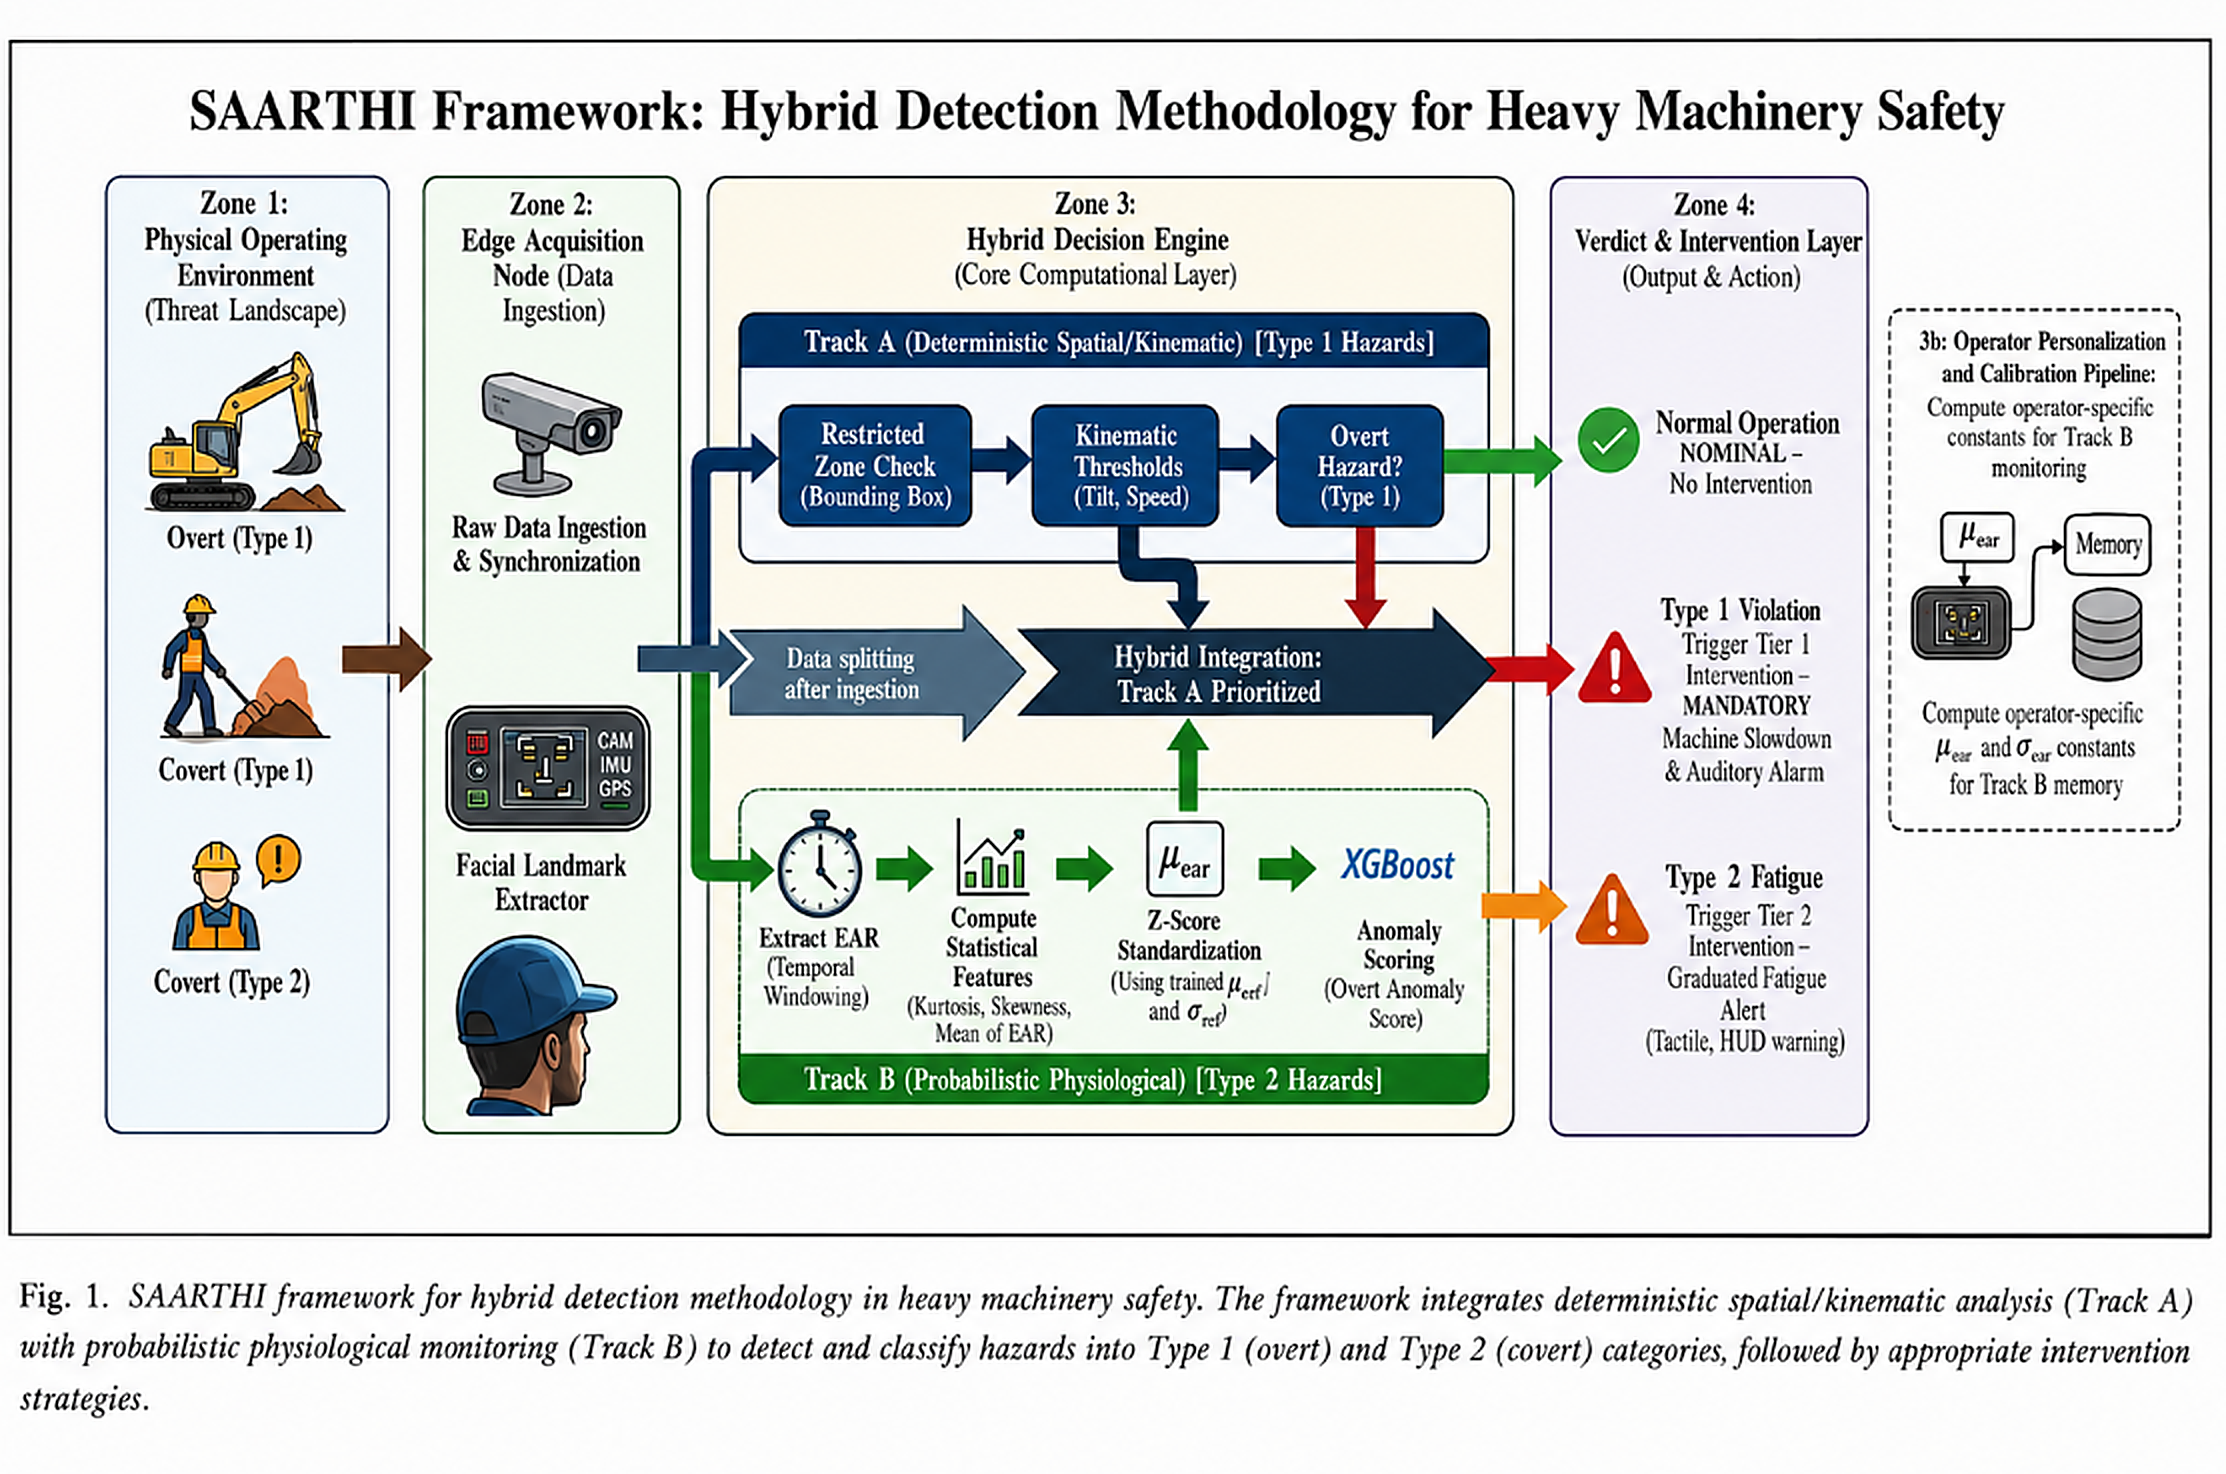
\includegraphics[width=\textwidth]{figures/framework_architecture.png}
\caption{SAARTHI framework for hybrid detection methodology in heavy machinery safety. The framework integrates deterministic spatial/kinematic analysis (Track A) with probabilistic physiological monitoring (Track B) to detect and classify hazards into Type 1 (overt) and Type 2 (covert) categories, followed by appropriate intervention strategies.}
\label{fig:framework}
\end{figure*}

\begin{itemize}
\item \textbf{Zone 1 --- Operating Environment:} The physical threat landscape: the
overt (Type~1) and covert (Type~2) hazards present in and around the heavy
machine.
\item \textbf{Zone 2 --- Edge Acquisition Node:} Raw data ingestion through the
cabin-facing camera and the machine's telemetry interface (e.g.\ the CAN bus).
\item \textbf{Zone 3 --- Hybrid Decision Engine:} The core computational layer, housing
Track~A (deterministic spatial/kinematic rules) and Track~B (XGBoost
physiological anomaly scoring).
\item \textbf{Zone 4 --- Verdict \& Intervention:} The final decision layer, which
outputs the real-time safety status and manages the appropriate Tier-1 or
Tier-2 response.
\end{itemize}

End to end, the pipeline runs in four steps:

\begin{enumerate}
\item \textbf{Ingestion.} Raw video frames and machine telemetry are captured
and synchronized.
\item \textbf{Buffering.} EAR values and machine states accumulate in a size-$w$
circular buffer, forming temporal sliding windows.
\item \textbf{Filtration (Track A).} Visual bounding boxes and kinematic
telemetry (speed, tilt) are checked against deterministic safety constraints
such as restricted-zone violations.
\item \textbf{Verification (Track B).} If Track~A raises no overt hazard, the
statistical physiological features (kurtosis, skewness, rate of change) are
computed and passed to the XGBoost model for covert fatigue scoring.
\end{enumerate}

Splitting the cheap work from the expensive work is the whole point of this
design. By keeping deterministic spatial and kinematic checks (Track~A) separate
from the heavier statistical physiological analysis (Track~B), the system spends
its machine-learning budget only where it is needed. The result is a lower
computational load on the edge device, which keeps thermal throttling at bay and
preserves real-time responsiveness without sacrificing diagnostic precision.

\subsection{Data Acquisition and Adaptive Preprocessing}

The data flow starts in Zone~2, where the cabin-facing camera and the telemetry
bus run continuously. This passive style of monitoring reflects the
non-intrusive philosophy that heavy machinery demands: it sidesteps the
``observer effect,'' since the operator is never asked to check in and is never
pulled away from a delicate task. And rather than processing every frame
indiscriminately, as a standard vision pipeline would, the SAARTHI node
selectively intercepts and synchronizes facial landmarks with CAN bus telemetry.

Because this multi-modal stream arrives fast and the device's SRAM is limited,
the system buffers it in a circular queue. The buffer acts as a shock absorber,
decoupling the irregular rate at which vision primitives are extracted from the
steady clock of the downstream inference engine.

\subsubsection{Circular Buffer Management}

Algorithm~\ref{alg:ingestion} formalizes how the stream is managed. Only valid
frames --- those with an intact face detection and high-confidence landmarks ---
are admitted. To avoid memory fragmentation, a persistent headache on embedded
targets, the buffer allocates its memory statically and overwrites in place,
always favouring the most recent temporal window.

\subsubsection{Feature Engineering and Statistical Standardization}

Once the temporal buffer $B_t$ holds a full window of valid samples, the system
moves into feature engineering. The main challenge here is taming the stochastic
variance in the physiological and kinematic readings, so that the feature vector
$\mathbf{x}$ handed to the classifier is stable enough to trust.

\begin{algorithm}[h]
\caption{Adaptive Rolling Window Data Ingestion}
\label{alg:ingestion}
\KwIn{Raw video stream $S_V$, telemetry stream $S_T$, window size $w$}
\KwOut{Temporal buffer $B_t$}
\Globals{Static ring buffer $R$ of size $w$, head pointer $p$}
\While{System Active}{
    $f_{raw} \gets \mathrm{ReadFrame}(S_V)$\;
    $t_{raw} \gets \mathrm{ReadTelemetry}(S_T)$\;
    \tcp{Stage 1: detection integrity filtering}
    \If{$\mathrm{DetectFace}(f_{raw}) = \textsc{fail}$}{
        \textbf{continue}\tcp*{discard frames lacking a clear face}
    }
    \tcp{Stage 2: extraction}
    $e_{ear} \gets \mathrm{ExtractEAR}(f_{raw})$\;
    $k_{state} \gets \mathrm{ExtractKinematics}(t_{raw})$\;
    \tcp{Stage 3: buffer injection}
    $R[p] \gets \{\, e_{ear},\ k_{state},\ \text{timestamp} \,\}$\;
    $p \gets (p + 1) \bmod w$\;
    \tcp{check window saturation}
    \If{$p = 0$ \textbf{\emph{or}} \textsc{BufferFullFlag}}{
        $B_t \gets \mathrm{Linearize}(R)$\;
        \textbf{Trigger} $\mathrm{FeatureExtraction}(B_t)$\;
    }
}
\end{algorithm}

\subsubsection{Window Size Selection and Stability Criterion}

Choosing the window size $w$ is a metrological trade-off between detection
latency and statistical stability. Empirically, raw detection accuracy peaks at
smaller windows --- but that peak sits squarely in the white-noise-dominated
regime, where frame-to-frame variance (from natural rapid blinks, for example)
runs high. Short windows may look accurate on paper, yet they invite false
positives driven by transient physiological noise.

To put the choice on firmer ground, we ran an Allan deviation analysis over
steady-state operator streams. The noise floor bottomed out at an averaging time
of $\tau_{opt} \approx 30.0$ samples --- the stability plateau, where white noise
is already minimized but random-walk drift (posture shifts and the like) has not
yet taken over. SAARTHI therefore uses $w = 30$, sitting right at $\tau_{opt}$
and trading the marginal sensitivity of smaller windows for operational
stability. At this size the total data-collection time stays under 1.5 seconds,
comfortably inside the $T_{hazard\_onset}$ pre-intervention budget.

\subsubsection{Z-Score Standardization}

XGBoost's decision space is distance-sensitive, and our feature space is
heterogeneous, so the features have to be scaled. Left unscaled, high-magnitude
variables like variance would swamp low-range ones like skewness and tilt the
decision boundary. The system applies Z-score standardization in real time:

\begin{equation}
z_i = \frac{x_i - \mu_{cal}}{\sigma_{cal}}
\label{eq:zscore}
\end{equation}

The constants $\mu_{cal}$ and $\sigma_{cal}$ are fixed during the initial
30-second operator calibration and kept in memory, which spares the device from
recomputing global statistics on every frame. Algorithm~\ref{alg:features}
spells out the full extraction logic.

\begin{algorithm}[h]
\caption{Statistical Feature Extraction}
\label{alg:features}
\KwIn{Temporal buffer $B_t$, calibration stats $(\mu_{cal}, \sigma_{cal})$}
\KwOut{Normalized feature vector $\mathbf{z}$}
\tcp{Compute raw mean (first pass)}
$\mu \gets 0$\;
\For{$i \gets 1$ \KwTo $w$}{
    $\mu \gets \mu + B_t[i].\mathrm{ear}$\;
}
$\mu \gets \mu / w$\;
\tcp{Compute higher-order moments (second pass)}
$\mathit{sum\_sq} \gets 0$;\quad $\mathit{sum\_cu} \gets 0$;\quad $\mathit{sum\_qd} \gets 0$\;
\For{$i \gets 1$ \KwTo $w$}{
    $\mathit{diff} \gets B_t[i].\mathrm{ear} - \mu$\;
    $\mathit{sum\_sq} \gets \mathit{sum\_sq} + \mathit{diff}^2$\;
    $\mathit{sum\_cu} \gets \mathit{sum\_cu} + \mathit{diff}^3$\;
    $\mathit{sum\_qd} \gets \mathit{sum\_qd} + \mathit{diff}^4$\;
}
$\sigma \gets \sqrt{\mathit{sum\_sq} / (w - 1)}$\;
$E_{roc} \gets B_t[w].\mathrm{ear} - B_t[w-5].\mathrm{ear}$\;
$S_k \gets (\mathit{sum\_cu} / w) / \sigma^3$\;
$K_u \gets \big((\mathit{sum\_qd} / w) / \sigma^4\big) - 3$\tcp*{excess kurtosis}
\tcp{Construct and standardize}
$\mathbf{x} \gets [\,\mu,\ \sigma,\ E_{roc},\ S_k,\ K_u\,]$\;
\For{$j \gets 1$ \KwTo $5$}{
    $z[j] \gets (x[j] - \mu_{cal}[j]) / \sigma_{cal}[j]$\;
}
\Return $\mathbf{z}$\;
\end{algorithm}

\subsection{Track A: Deterministic Spatial and Kinematic Verification}

Track~A is a fast, deterministic pre-filter that runs in $O(1)$. Its job is to
catch Type~1 overt hazards the instant they occur --- a pedestrian entering a
restricted zone, an unsafe machine tilt --- with no machine-learning overhead at
all. It does this by testing the current state against a deterministic
constraint set $C_{rules}$, implemented as a lookup over predefined spatial
boundaries and kinematic thresholds.

Bounding-box intersection tests and threshold comparisons cost next to nothing
on any edge processor, so this gate is cheap. Only states that clear Track~A ---
those with no deterministic hazard --- go on to Track~B for the deeper
physiological analysis.

\subsection{Track B: Statistical Physiological Anomaly Scoring (XGBoost)}

Track~B takes on the Type~2 covert hazard, the case where the operator still
looks awake and engaged while the underlying physiological signal quietly drifts
toward fatigue. To catch that drift, the system uses a gradient-boosted ensemble
(XGBoost) trained on the standardized feature vector $\mathbf{z}$.

Most classifiers need labelled ``fatigue'' examples, which are expensive or
simply unavailable for every individual operator. SAARTHI sidesteps that: the
calibration phase learns a personalized envelope of normal operation for each
operator, and any feature vector that strays well outside that envelope is
flagged as a fatigue anomaly.

\subsubsection{The Primal and Dual Formulations}

The ensemble's goal is to carve a decision boundary in the feature space
$\Phi(\mathbf{x})$ that separates the bulk of the training data --- alert
operator states --- from the anomalous region. It does so by learning an
additive ensemble of $T$ weak learners that minimizes a regularized objective:

\begin{equation}
\mathcal{L} = \sum_{i=1}^{n} l(y_i, \hat{y}_i) + \sum_{t=1}^{T} \Omega(f_t)
\end{equation}

where $l$ is the loss, $\hat{y}_i$ the predicted score, and
$\Omega(f_t) = \gamma T + \tfrac{1}{2}\lambda \lVert w \rVert^2$ a penalty on
tree complexity. SAARTHI sets $\lambda = 1.0$ for strict regularization, treating
the outermost 1\% of training samples as candidate edge-case fatigue anomalies.

\subsubsection{The Gradient Boosting Kernel}

A linear boundary cannot capture the tangled, non-linear interplay between
higher-order moments like kurtosis and skewness. To build a surface expressive
enough to resolve them, XGBoost grows trees over the feature space
$\Phi(\mathbf{x})$, in effect approximating a kernel mapping. At inference time
the decision function is:

\begin{equation}
D(\mathbf{z}) = \operatorname{sgn}\!\left( \sum_{t=1}^{T} \eta \cdot f_t(\mathbf{z}) - \rho \right)
\label{eq:decision}
\end{equation}

where $\eta$ is the learning rate and $\rho$ the decision threshold. The
regularizer's $\gamma$ sets the minimum gain a split must earn, which in turn
governs how sharply the boundary curves. Algorithm~\ref{alg:training} outlines
the offline procedure that produces the boosted model shipped to the edge device.

\begin{algorithm}[h]
\caption{Offline Training Procedure}
\label{alg:training}
\KwIn{Training dataset $X_{train}$, params $(\eta, \lambda, \gamma, T)$}
\KwOut{Boosted model $M$, offset $\rho$}
\tcp{Feature matrix computation}
$Z \gets \mathrm{ExtractAndStandardize}(X_{train})$\;
\tcp{Ensemble training}
$M \gets \mathrm{XGBoost.Train}(Z,\ \mathrm{params}(\eta, \lambda, \gamma, T))$\;
\tcp{Extract decision threshold}
$\rho \gets \mathrm{ComputeThreshold}(M, X_{train})$\;
\tcp{Model compression for edge}
$M \gets \mathrm{Quantize}(M, \rho)$\;
\Return $M$\;
\end{algorithm}

When $D(\mathbf{z}) = -1$, the feature vector lies outside the calibrated
operator's learned envelope, and a fatigue alert is raised.

\subsubsection{Hybrid Logic Integration}

At the heart of Zone~3, the final decision logic fuses the deterministic
certainty of Track~A with the probabilistic rigour of Track~B;
Algorithm~\ref{alg:hybrid} lays out the combined flow. Running the lightweight
Track~A check first keeps the heavier XGBoost inference of Track~B on a low duty
cycle.

The final safety verdict is recovered through the ensemble's decision function
in Equation~\eqref{eq:decision}. If $D(\mathbf{z}) = -1$, the signal has fallen
outside the calibrated operator's normal distribution, and a Tier-2 fatigue
intervention fires.

\begin{algorithm}[h]
\caption{Hybrid Execution Flow}
\label{alg:hybrid}
\KwIn{Feature vector $\mathbf{z}$, kinematic state $k_{state}$, rules
$C_{rules}$, model $M$, threshold $\rho$}
\KwOut{Safety verdict $V$, intervention tier}
\tcp{Track A: deterministic gate}
\If{$\mathrm{CheckConstraints}(k_{state}, C_{rules}) = \textsc{violation}$}{
    $V \gets \textsc{hazard\_type\_1}$\;
    \textbf{Trigger} $\mathrm{Tier1Intervention}()$\;
    \Return $V$\;
}
\tcp{Track B: physiological anomaly scoring}
$\mathit{score} \gets \sum_{t=1}^{T} \eta \cdot f_t(\mathbf{z})$\;
\eIf{$\operatorname{sgn}(\mathit{score} - \rho) = -1$}{
    $V \gets \textsc{hazard\_type\_2}$\;
    \textbf{Trigger} $\mathrm{Tier2Intervention}()$\;
}{
    $V \gets \textsc{nominal}$\;
}
\Return $V$\;
\end{algorithm}

\subsection{Tiered Intervention Protocol}

When either track returns a positive verdict, SAARTHI responds with a
structured, tiered protocol rather than a single binary alarm. The graduation
matters in a heavy-machinery setting: a sudden, jarring alert in the middle of a
delicate manoeuvre --- a precise crane lift, say --- could itself cause the
accident it was meant to prevent.

\medskip
\noindent\textbf{Tier 1 --- Deterministic override (Track A).} Fires the instant
a kinematic violation is confirmed --- for example $\theta > \theta_{crit}$ while
$v \neq 0$, or a bounding-box intrusion into a restricted zone. The response is
non-negotiable: a mandatory speed-reduction command goes straight to the CAN bus
and a loud cabin alarm sounds. This tier is independent of operator behaviour or
any machine-learning state.

\medskip
\noindent\textbf{Tier 2 --- Adaptive fatigue alert (Track B).} Fires when
$D(\mathbf{z}) = -1$, signalling a sustained drift outside the operator's normal
envelope. Here the response builds gradually: first a tactile seat-vibration
pulse, then a visual HUD warning if the anomalous state persists beyond
$\delta_t$ consecutive windows. Should the operator not acknowledge within a
preset timeout $T_{ack}$, the system escalates to a Tier-1-equivalent mandatory
slow-down.

\medskip
This restrictive admission-control approach keeps interruptions rare during
normal operation while guaranteeing that genuine hazards always draw an
immediate, deterministic response --- which, in practice, is what earns operator
trust and keeps the system in use.

\subsection{Operator Personalization and Calibration}

Population-level fatigue models share one fundamental weakness: physiology varies
from operator to operator. A naturally narrow-eyed operator's baseline EAR mean
$\mu_{alert}$ can look, statistically, like another operator's fatigued state ---
and the resulting stream of false positives steadily erodes trust in the system.

SAARTHI answers this with a mandatory 30-second calibration at the start of every
shift. The operator is asked to look ahead, relaxed and alert, while the system
ingests $N_{cal}$ frames and computes operator-specific statistics:

\begin{equation}
\mu_{cal} = \frac{1}{N_{cal}} \sum_{i=1}^{N_{cal}} e_i,
\qquad
\sigma_{cal} = \sqrt{\frac{1}{N_{cal}-1} \sum_{i=1}^{N_{cal}} (e_i - \mu_{cal})^2}
\end{equation}

These constants then Z-score-normalize every incoming feature vector
(Equation~\ref{eq:zscore}), anchoring the whole pipeline to the individual's
physiology rather than a generic population mean. Each profile is saved to the
operator profile store, so returning operators skip re-calibration --- though the
profile can still be refreshed over time to track long-term physiological drift.


% !TEX root = ../main.tex

\section{Experimental Setup}

Evaluating SAARTHI meant answering three separate questions: does the detection
logic work, can it be trusted statistically, and will it actually run on the
hardware we intend to put in a cab? This section walks through the dataset we
built on, the protocol we used to synthesize fatigue signatures that do not
exist in any public corpus, and the cross-validation scheme that keeps the
reported numbers honest.

\subsection{Dataset Characteristics and Preprocessing}
We built the evaluation on a tailored subset of the NTHU Driver Drowsiness
Dataset (NTHU-DDD). Of the candidates we considered, NTHU-DDD came closest to
the messy reality of a machine cab: a dense collection of operator states
recorded under genuinely awkward conditions, with the kind of physiological
variation that laboratory captures tend to iron out. Table
\ref{tab:dataset_census} gives the census of the subset used for training and
validation.

The mess is the point. A perfectly lit lab dataset, with facial landmarks
tracked under ideal conditions, teaches a model very little about shadows,
head-pose swings, sunglasses, or the plain fact that people's faces differ.
NTHU-DDD contains all of these, and that variance is what forces the model to
learn the difference between an ordinary rapid blink and the slower
physiological drift that marks the onset of fatigue.

\begin{table}[htbp]
\centering
\caption{Dataset census. The evaluation drew on a large subset of NTHU-DDD ---
large enough, in our judgement, to support the statistical claims made in
Section VI.}
\label{tab:dataset_census}
\begin{tabular}{lr}
\toprule
\textbf{Metric} & \textbf{Count} \\
\midrule
Total Raw EAR Samples (Frames) & 450,194 \\
Unique Subjects (Operators) & 22 \\
Distinct Lighting Conditions & 4 \\
Distinct Temporal Sequences & 465 \\
\bottomrule
\end{tabular}
\end{table}

\subsubsection{Preprocessing Pipeline}
Before any features were extracted, the raw video stream went through a
cleaning pass deliberately kept simple enough for a low-power edge device to
reproduce. Where facial landmarks dropped out --- a hand passing over the face,
an extreme head turn --- we forward-filled the gap rather than discard the
sequence, preserving temporal continuity. The cleaned stream was then cut into
rolling windows of size $w = 30$, the value fixed by the stability analysis in
Section IV.

\subsection{Synthetic Hazard Injection Protocol}
Here we ran into a problem that anyone working in industrial safety will
recognize: there is no public dataset of labelled fatigue accidents involving
heavy machinery, and there is no ethical way to produce one --- nobody is going
to let a drowsy operator keep driving an excavator for the sake of a label. So
we injected the hazards ourselves, mathematically.

The idea is to take legitimate, alert physiological signals and perturb them
into micro-sleep and deep-fatigue signatures whose magnitude and duration we
control exactly. Want a prolonged eye closure, or an erratic head drop? Dial it
in. The simulation can then model operators at any point along the fatigue
curve, from barely-detectable early drowsiness to the late stage that precedes
an accident.

\subsubsection{Track A Injection: Overt Kinematic Violations}
Track A deals in hazards the machine itself can report: a boom arm pushed past
its safe operating angle, a travel-speed violation mid-slew, a cab tilted
beyond its stability limit. None of this correlates with the operator's
physiology --- the EAR signal stays untouched --- yet each event demands an
immediate, deterministic response.

We simulate three normalised CAN-bus sensor channels:
\begin{itemize}
    \item \textbf{$s_0$: Boom Angle} (threshold $> 0.85$)
    \item \textbf{$s_1$: Travel Speed} (threshold $> 0.90$)
    \item \textbf{$s_2$: Cab Tilt} (threshold $> 0.80$)
\end{itemize}
In normal operation each channel behaves as $s_c \sim
\mathcal{N}(\mu_c^{\text{safe}}, \sigma_c^2)$, with the safe means held a full
three standard deviations below the alarm thresholds; during a violation
event, at least one channel is driven past its limit. Every channel also
carries Gaussian ADC noise ($\sigma_{\text{noise}} = 0.02$) --- the
quantisation artefacts and vibration-induced jitter that a sensor bolted to a
working excavator cannot avoid.

Violations enter at a $5\%$ window-level rate, which works out to roughly two
non-overlapping events per 1{,}000-frame session, each spanning $w = 30$
frames. Detection is deliberately unglamorous: the rule takes the mean sensor
reading across the window and fires if any channel mean clears its threshold.
That $w$-frame averaging is a standard debounce --- it shrugs off
single-sample ADC glitches while still guaranteeing a detection latency of at
most one window.

\subsubsection{Track B Injection: Covert Fatigue Onset}
Testing the XGBoost physiological model called for a subtler adversary: an
operator who sails through every deterministic Track A check while quietly
succumbing to micro-behavioural fatigue. Fatigue episodes of this kind are rare
in continuous industrial work, so we kept the injection rate conservative at
3\%, split as follows:
\begin{itemize}
    \item \textbf{Micro-Sleeps (2\%):} Short but profound eye closures, lasting
    anywhere from 1.0 to 2.5 seconds.
    \item \textbf{Physiological Drift (1\%):} A gradual slowing of the blink
    rate paired with erratic head-pose variation --- the classic early
    signature of drowsiness.
\end{itemize}

The perturbed signal $E_{anom}(t)$ comes from a linear transformation of the
normal baseline EAR signal $E_{norm}(t)$:
\begin{equation}
    E_{anom}(t) = (E_{norm}(t) \cdot k_v) + k_o
\end{equation}
where $k_v$ scales the variance (droopy eyelid dynamics) and $k_o$ is an
additive offset (a sustained drop in baseline eye openness).

Real operators do not simply switch from alert to asleep; they fatigue
progressively, and often try to mask it. To capture that, both parameters are
driven by a perturbation magnitude $\delta \in [0, 1]$:
\begin{align}
    k_v &= 1 - (\delta \cdot \mathcal{U}(0.1, 0.3)) \\
    k_o &= -\delta \cdot \mathcal{U}(0.05, 0.15)
\end{align}
with $\mathcal{U}$ a uniform random distribution. The formulation matters: it
makes the anomalies degrade the way real physiology degrades, rather than
adding white noise and calling it fatigue. A high $\delta$ corresponds to
late-stage drowsiness --- heavy head bobbing, long eye closures --- while a low
$\delta$ gives the faint early onset that is genuinely hard to catch.

Figure \ref{fig:temporal_distribution} shows where the injected anomalies land
in time, over the first twelve sessions of the actual evaluation stream. Two
regimes are visible at once. Micro-sleeps arrive as short, sharp bursts ---
profound EAR depressions that come and go within a couple of seconds --- while
the drift segments stretch out far longer, dragging the baseline downward for
sustained periods. Because every frame touched by a perturbation is labelled
anomalous, this drift coverage is also what produces the high window-level
anomaly rate ($\approx 88.8\%$) that the class-imbalance analysis in
Section~VII has to contend with. The environment the classifier faces is, by
construction, dynamic and non-stationary.

\subsection{Model Configuration and Hyperparameters}

\begin{figure*}[t]
\centering
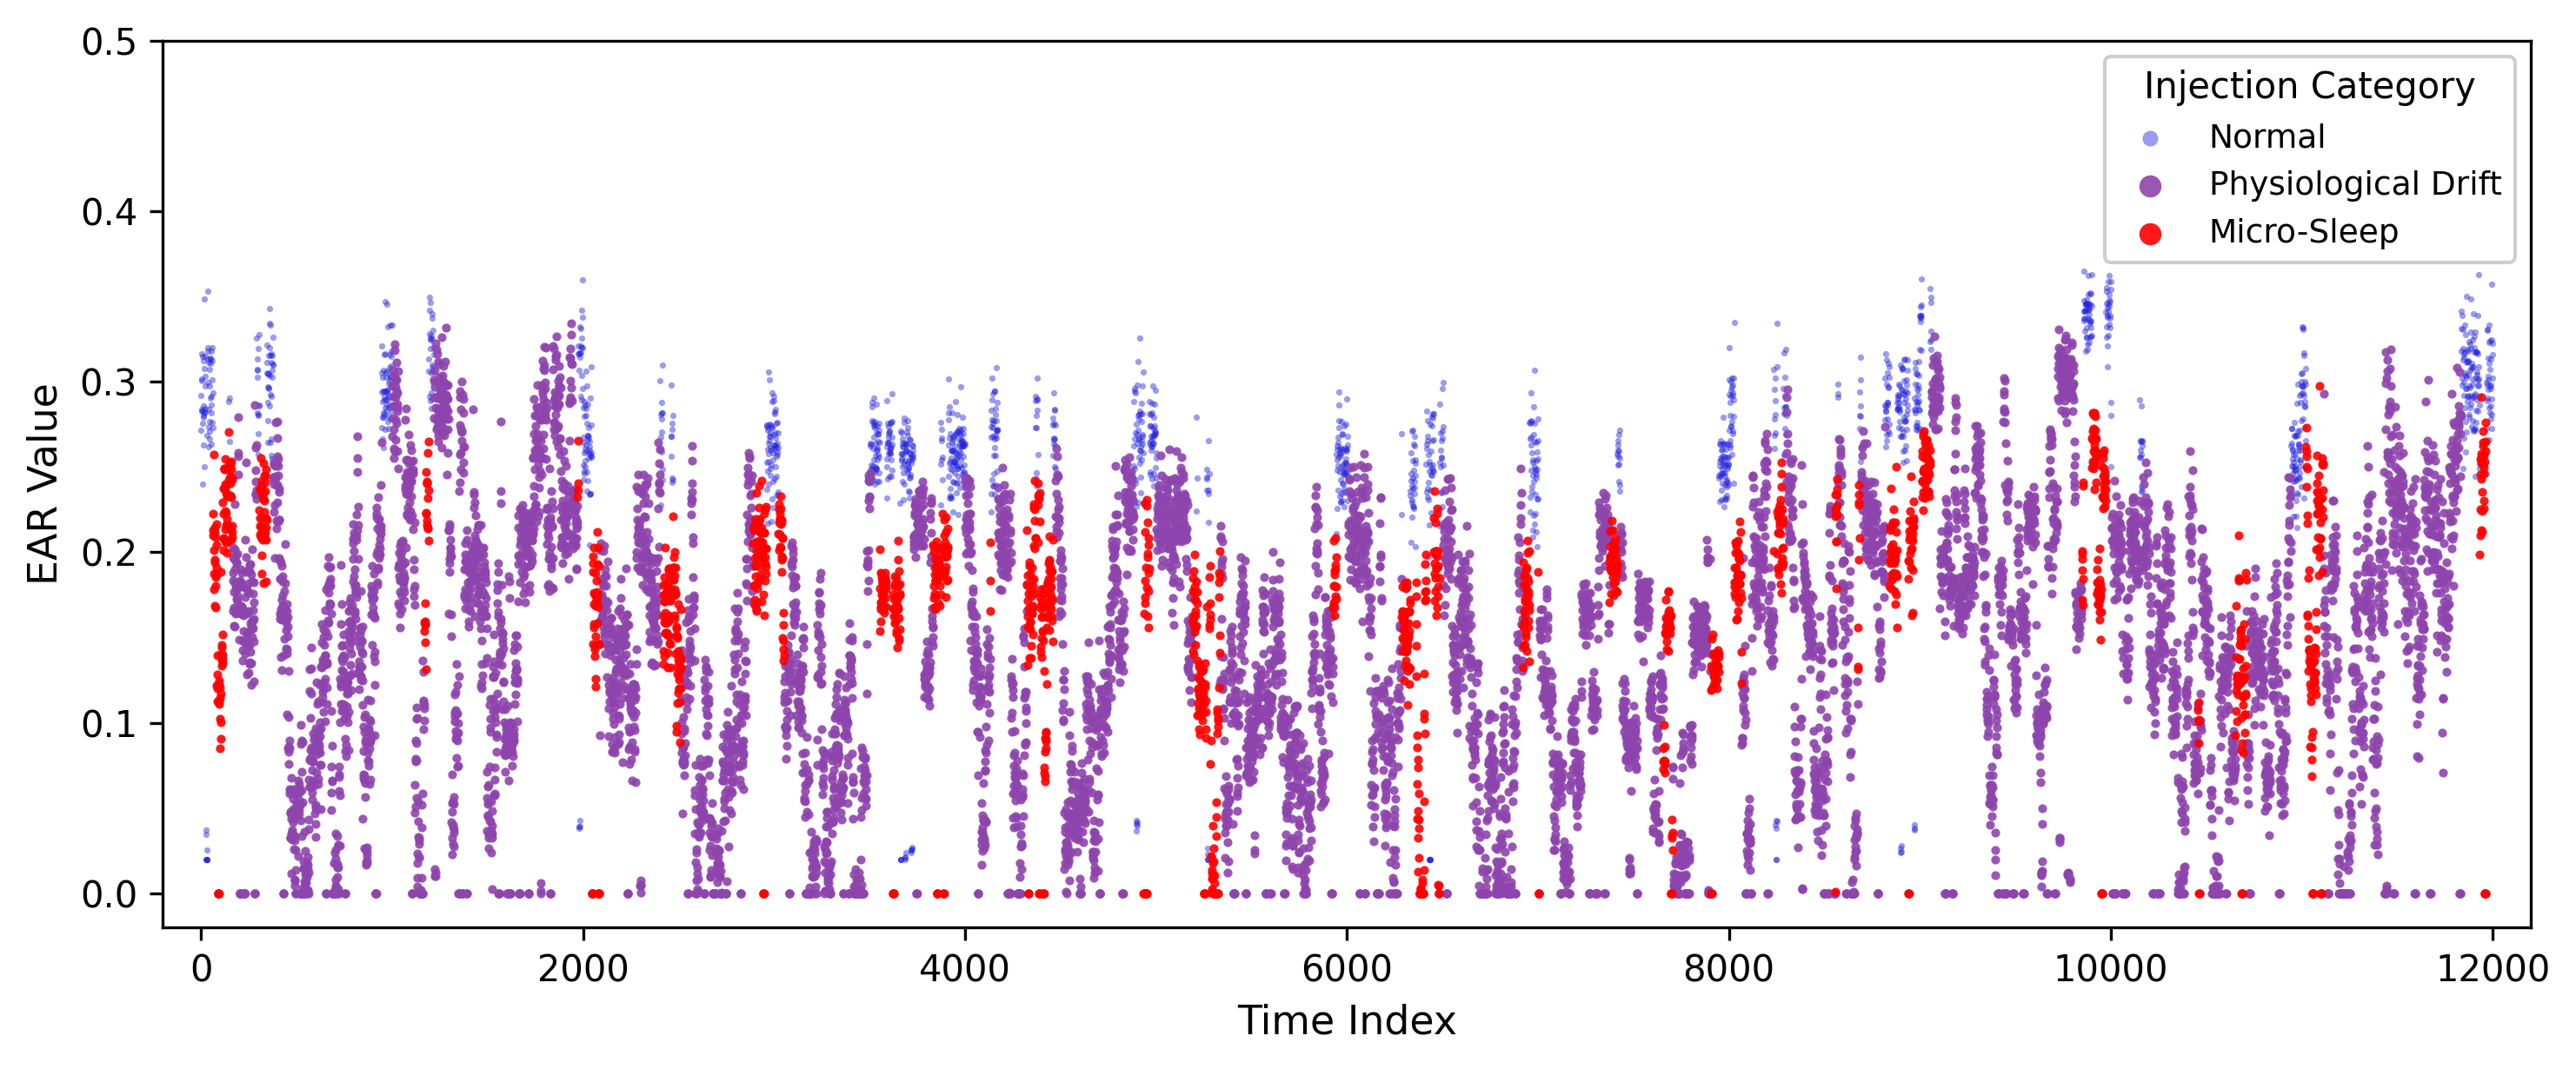
\includegraphics[width=\textwidth]{figures/temporal_distribution.png}
\caption{Temporal distribution of injected hazards over the first twelve
sessions of the evaluation stream (12{,}000 frames, $\delta = 0.5$,
\texttt{SEED=42}). `Micro-Sleep' bursts (red) appear as short, transient EAR
depressions, while `Physiological Drift' segments (purple) suppress the
baseline over sustained stretches; the `Normal' alert baseline (blue) sits
above both. The transient character of the micro-sleep events is why the
$w=30$ sliding window matters: a longer window would smooth these short
bursts out of existence.}
\label{fig:temporal_distribution}
\end{figure*}

We tuned the SAARTHI XGBoost classifier by grid search over a subset of clean,
alert training data. The target was a tight, personalized decision envelope
that still retains the bulk of normal operational samples --- err too far in
either direction and the system becomes either deaf to fatigue or unbearable to
work under. Table \ref{tab:hyperparameters} lists the parameters we settled on.

For the deep learning baselines we used a Denoising Autoencoder (DAE), kept
deliberately small so the comparison stays fair. The network passes the
5-dimensional feature vector through an Encoder
($5 \rightarrow 16 \rightarrow$ Batch Norm (BN) $\rightarrow$ ReLU
$\rightarrow 8$) and a mirrored Decoder
($8 \rightarrow 16 \rightarrow$ BN $\rightarrow$ ReLU $\rightarrow 5$).

\subsubsection{Feature Orthogonality Check}
One question worth settling before training: do the five features actually
carry independent information, or are we feeding the model the same signal five
times? Figure \ref{fig:feature_correlation} shows the feature correlation
matrix.

\begin{figure}[htbp]
\centering
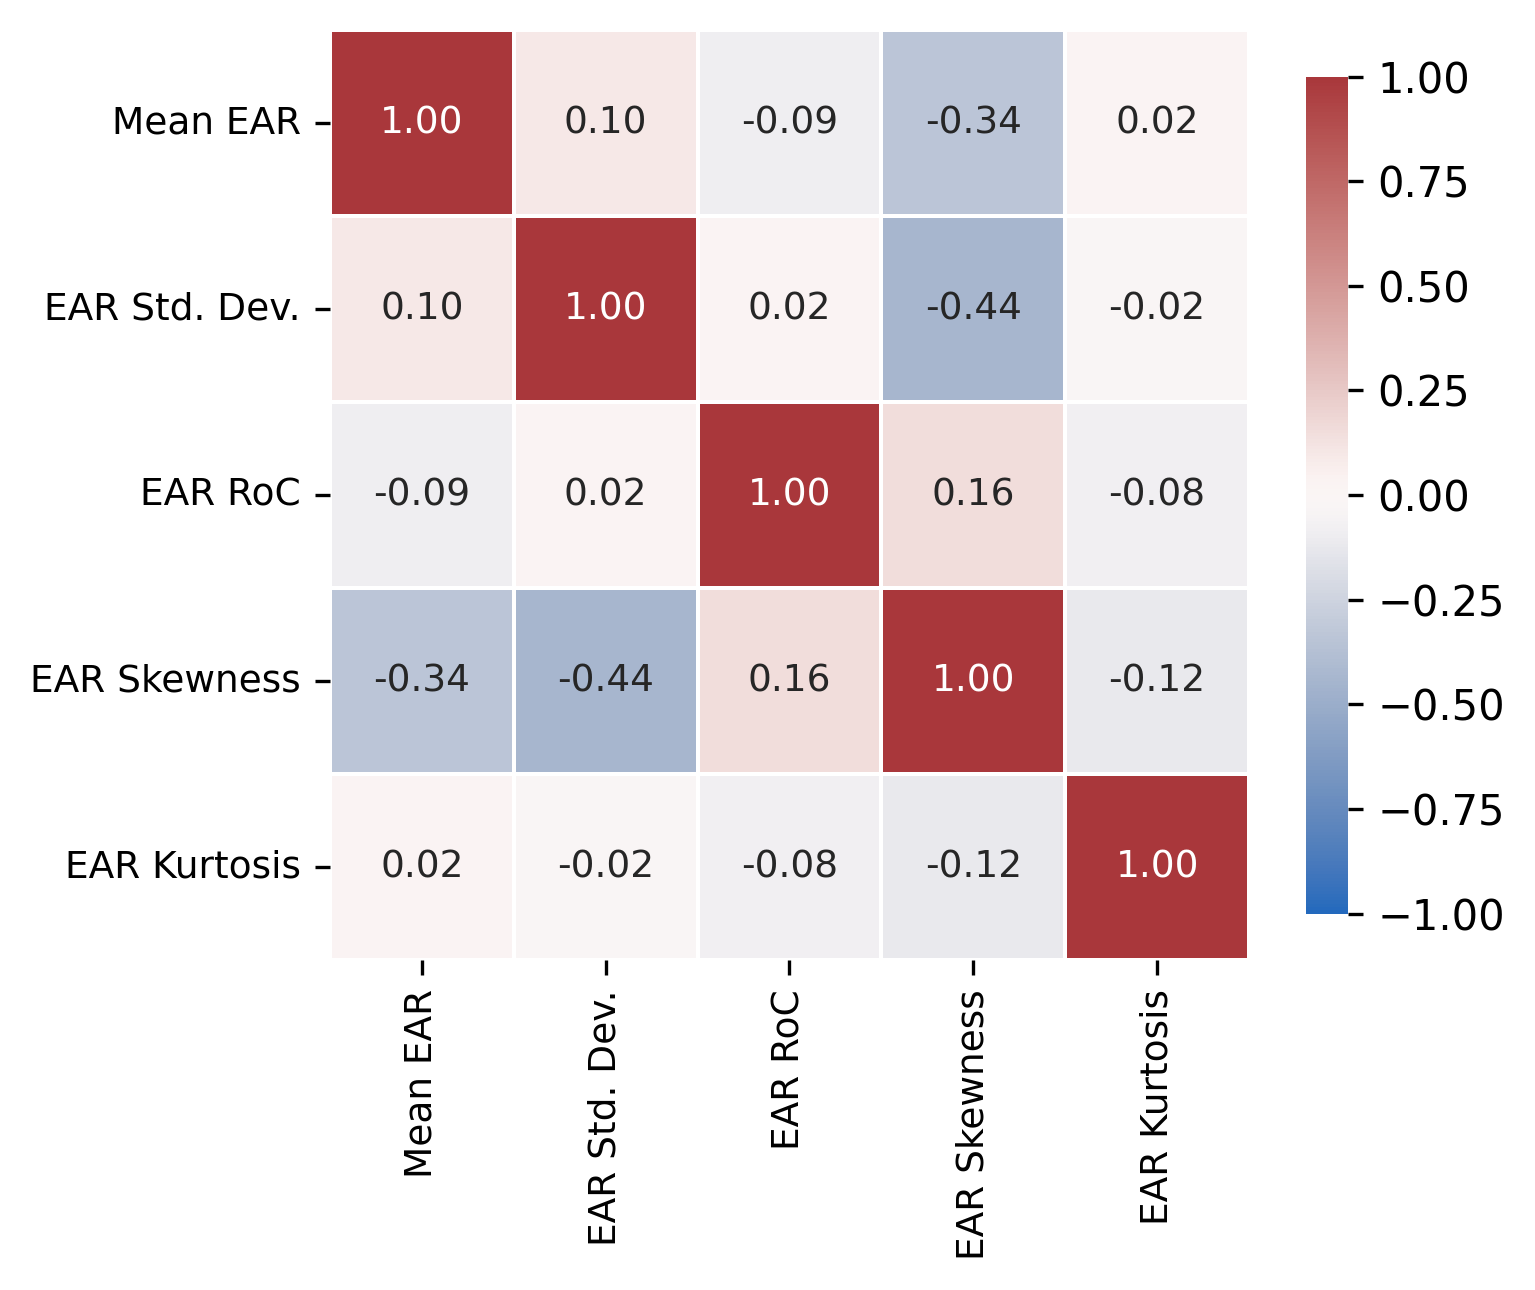
\includegraphics[width=\columnwidth]{figures/feature_correlation.png}
\caption{Feature orthogonality (computed from the full 451{,}515-window
dataset, SEED = 42). The largest off-diagonal correlation is
$r = -0.44$ between Std.\ Dev.\ and Skewness; all remaining pairs
stay below $|r| = 0.35$. No two features carry the same
physiological information.}
\label{fig:feature_correlation}
\end{figure}

To put a number on that independence, we ran a Variance Inflation Factor (VIF)
analysis. The worst offender was Skewness at a VIF of 1.46 --- well within the
acceptable range below the standard trouble threshold of 5.0 (individual VIFs:
Mean EAR 1.14, Std.\ Dev.\ 1.27, $E_{roc}$ 1.04, Skewness 1.46, Kurtosis 1.03).
Each of the five statistical moments therefore contributes its own physiological
evidence to the XGBoost decision boundary rather than restating a neighbour's.

\begin{table}[htbp]
\centering
\caption{Simulation parameters and model configuration. The regularization is
deliberately strict: in a heavy-machinery safety context, a tight physiological
envelope that minimizes False Negatives is worth far more than a forgiving
one.}
\label{tab:hyperparameters}
\begin{tabular}{llp{3.8cm}}
\toprule
\textbf{Category} & \textbf{Parameter} & \textbf{Value / Description} \\
\midrule
\textbf{Dataset} & Source & NTHU-DDD \\
& Window Size ($w$) & 30 samples ($\approx 1.0$ sec) \\
\midrule
\textbf{SAARTHI} & Ensemble Size ($T$) & 100 Trees \\
\textbf{(XGBoost)} & Learning Rate ($\eta$) & 0.1 \\
& Regularization ($\lambda$) & 1.0 (Strict Outlier Tolerance) \\
\midrule
\textbf{Baselines} & Isolation Forest & Contamination=0.05, Trees=100 \\
& Autoencoder & Latent Dim=8, Epochs=50, LR=0.001 \\
\midrule
\textbf{Injection} & Track A Rate & 5\% (Overt Kinematic Hazards) \\
& Track B Rate & 2\% (Micro-Sleeps), 1\% (Physio. Drift) \\
& Perturbation ($\delta$) & Varied $[0.0, 1.0]$ for robustness test \\
\bottomrule
\end{tabular}
\end{table}

\subsection{Hardware Feasibility Benchmarking}
The latency figures reported in Section VI are only as good as their
reproducibility, so all performance benchmarks were run on a single,
standardized compute environment, detailed in Table
\ref{tab:hardware_benchmarks}.

\begin{table}[htbp]
\centering
\caption{Hardware benchmarking environment. All latency and memory figures
were measured directly on the benchmark host using 
\texttt{run\_experiment.py} (SEED = 42).}
\label{tab:hardware_benchmarks}
\begin{tabular}{llp{3.4cm}}
\toprule
\textbf{Category} & \textbf{Component} & \textbf{Specification} \\
\midrule
\textbf{Benchmark} & Processor & Intel Core Ultra 5 125U, 12C/14T @ 3.60 GHz \\
\textbf{Host} & Memory & 15.7 GB RAM \\
& OS & Windows 10 (Build 26200) \\
& Runtime & Python 3.11.9, XGBoost 3.0.2 \\
\midrule
\textbf{Target Edge} & SoC Class & ARM Cortex-A72 (Raspberry Pi 4 / Jetson Nano tier) \\
\textbf{Node} & Memory & 4 GB LPDDR4 \\
& Accelerator & None (CPU-only inference) \\
\midrule
\textbf{Deployed} & Footprint & 165.75 KB (pickle) / 206.79 KB (JSON) \\
\textbf{Model} & Inf.\ Latency & 0.55 ms mean, 0.98 ms p99 \\
\bottomrule
\end{tabular}
\end{table}

The question that actually decides deployment is whether the algorithm survives
on the resource-constrained edge nodes --- Raspberry Pi, the NVIDIA Jetson
series --- that get installed in machinery cabins. Cloud offloading was never an
option; the round-trip latency alone would defeat the purpose. The serialized
XGBoost ensemble occupies 165.75 KB in pickle format (206.79 KB as a portable
JSON booster), measured directly on the benchmark host. Both figures sit well
inside the RAM budget of this hardware class, leaving sufficient headroom for
the concurrent high-frequency video buffer and the CAN bus handlers.

The inference cost is equally manageable. On the benchmark host (Intel Core
Ultra 5 125U), a single 5-feature inference call completes in 0.55 ms on average
($p_{99} = 0.98$ ms). This is two orders of magnitude below the
$T_{\text{human}} \approx 250$ ms human reaction threshold, confirming that
SAARTHI's decision pipeline will never become the bottleneck in the intervention
chain regardless of the edge SoC deployed by the fleet.

\subsection{Validation Methodology}
All results were produced under 10-Fold Stratified Cross-Validation with a
fixed global random seed. Stratification matters here more than usual: hazard
events are rare by construction, and an unstratified split can hand a lazy
classifier an inflated accuracy score simply by starving some folds of
positives. Partitioning so that the Alert-Baseline-to-Fatigued/Hazardous ratio
stays constant across folds closes that loophole. Every metric reported in this
paper is the mean over 10 independent simulation runs.


% !TEX root = ../main.tex
% All numerical results in this section are computed values from:
%   experiments/run_experiment.py  (SEED=42, w=30, 10-fold stratified CV)
%   Full output: experiments/results/saarthi_results.json

\section{Results and Performance Analysis}

SAARTHI was run through the synthetic injection protocol of Section~V in full:
451{,}515 feature windows across 465 operator sessions, with a fixed seed
(SEED = 42) and $w = 30$ throughout. Every number reported below is the mean
$\mu$ and standard deviation $\sigma$ over ten independent stratified
cross-validation folds --- nothing here rests on a single lucky split.

\subsection{Diagnostic Accuracy and Architecture Comparison}

Table~\ref{tab:comparative_metrics} lays out the key indicators for all four
architectures, and Figure~\ref{fig:hybrid_comparison} shows the same
comparison graphically. SAARTHI takes every column: an F1-Score of
$0.952 \pm 0.001$, an AUC of $0.932 \pm 0.002$, and an Average Precision of
$0.991 \pm 0.000$. The metric worth pausing on, though, is the Matthews
Correlation Coefficient of $0.505 \pm 0.008$. This dataset is heavily
imbalanced --- the anomaly rate sits near 88.8\% --- and on a skewed binary
problem, accuracy and even F1 can be flattered by simply siding with the
majority class. MCC cannot. A value around 0.5 here reflects genuine
discriminative power, not a class-majority bias dressed up as performance.

\begin{table}[htbp]
\centering
\caption{Comparative performance metrics (mean $\pm$ std over 10 folds).
All values are computed from \texttt{run\_experiment.py} with \texttt{SEED=42}.}
\label{tab:comparative_metrics}
\resizebox{\columnwidth}{!}{%
\begin{tabular}{lccccc}
\toprule
\textbf{Architecture} & \textbf{Acc} & \textbf{F1-Score} & \textbf{MCC} & \textbf{AUC} & \textbf{AP} \\
\midrule
Na\"ive (Threshold)        & $0.609{\pm}0.002$ & $0.719{\pm}0.002$ & $0.326{\pm}0.003$ & $0.884{\pm}0.002$ & $0.983{\pm}0.000$ \\
Hybrid (Isol.\ Forest)    & $0.248{\pm}0.017$ & $0.273{\pm}0.028$ & $0.097{\pm}0.014$ & $0.732{\pm}0.009$ & $0.947{\pm}0.003$ \\
Hybrid (Autoencoder)       & $0.603{\pm}0.017$ & $0.714{\pm}0.016$ & $0.322{\pm}0.013$ & $0.784{\pm}0.021$ & $0.970{\pm}0.003$ \\
\textbf{SAARTHI (XGBoost)} & $\mathbf{0.913{\pm}0.001}$ & $\mathbf{0.952{\pm}0.001}$ & $\mathbf{0.505{\pm}0.008}$ & $\mathbf{0.932{\pm}0.002}$ & $\mathbf{0.991{\pm}0.000}$ \\
\bottomrule
\end{tabular}%
}
\end{table}

\begin{figure*}[!t]
\centering
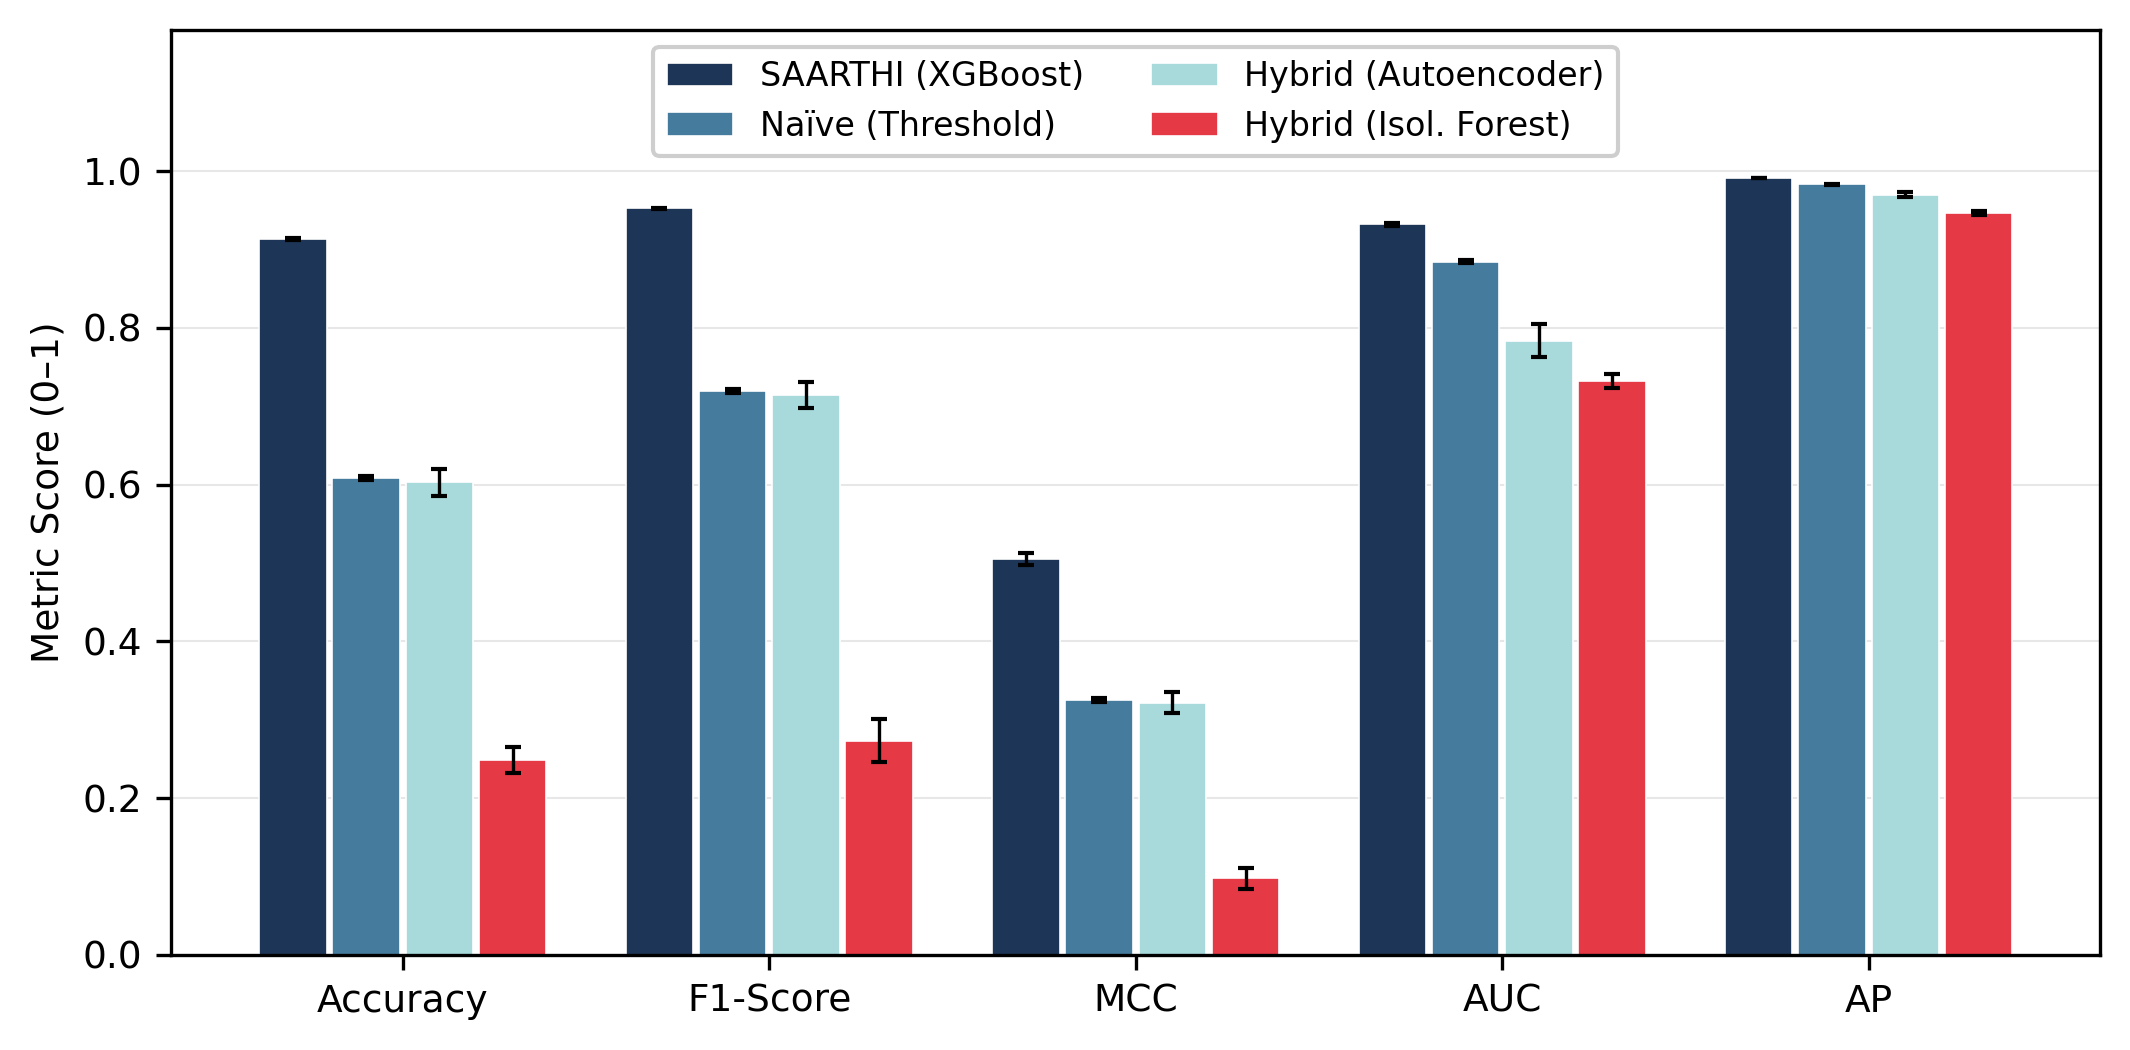
\includegraphics[width=\textwidth]{figures/hybrid_comparison.png}
\caption{Architecture comparison across all five metrics (mean over 10 folds;
error bars show one standard deviation). SAARTHI leads on every indicator,
with the widest margin on MCC --- the metric hardest to inflate on an
imbalanced dataset. The Isolation Forest's collapse at the operating threshold
is visible in its Accuracy and F1 despite a respectable AUC.}
\label{fig:hybrid_comparison}
\end{figure*}

The Isolation Forest deserves a closer look, because its failure is
instructive. Its AUC of 0.732 says the model ranks anomalies reasonably well;
its F1 of $0.273 \pm 0.028$ says that at the actual operating threshold, the
ranking is useless --- the confusion matrix is drowning in false positives
(336{,}824 FP against 63{,}921 TP across all folds). This is a known weakness
of tree-based density estimators on heavily imbalanced data: a single global
contamination parameter has no way to adapt to a physiological envelope that
differs from operator to operator. SAARTHI sidesteps the failure mode
entirely, because its 30-second calibration phase anchors every Z-score to the
individual's own baseline before inference ever begins.

The Autoencoder tells a different story. On F1 it roughly matches the na\"ive
threshold ($0.714 \pm 0.016$), but its AUC trails SAARTHI by 14.8 points ---
the discrimination surface it learns is simply less well-formed across
decision thresholds. Reconstruction error, it turns out, is not very sensitive
to the distributional shape features that characterize micro-sleep events;
a gradient-boosted boundary trained directly on the standardized feature
vector can split on them explicitly.

Figure~\ref{fig:confusion_matrix} shows SAARTHI's aggregated confusion matrix.
The model recovers 389{,}678 of the 400{,}745 anomalous windows (recall
$= 0.972$) while keeping precision at 0.933 --- the balance that produces the
0.952 F1.

\begin{figure}[htbp]
\centering
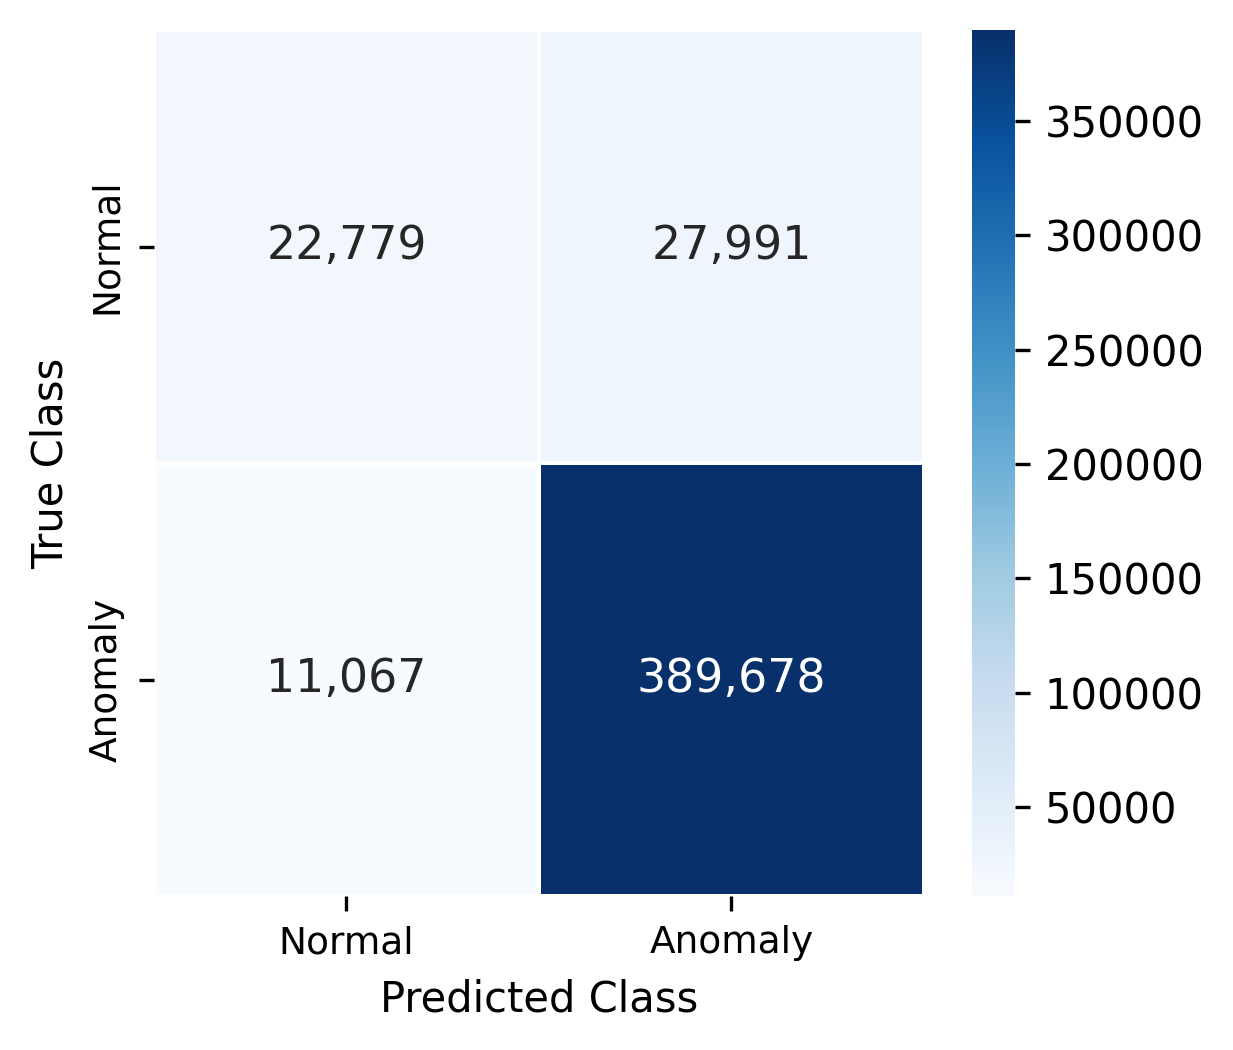
\includegraphics[width=0.85\columnwidth]{figures/confusion_matrix.png}
\caption{Aggregated confusion matrix for SAARTHI (XGBoost) across all folds.
Recall on anomalous windows reaches 0.972 at a precision of 0.933.}
\label{fig:confusion_matrix}
\end{figure}

\subsection{Statistical Significance and Reliability}

A lead in the mean is only interesting if it survives a significance test, so
we tested. A Friedman Chi-Squared test over the ten per-fold F1-Scores of all
four architectures rejects the hypothesis of equivalent performance
decisively ($\chi^2 = 27.12$, $p = 6 \times 10^{-6}$). The post-hoc Wilcoxon
signed-rank test against the next-best baseline (the na\"ive threshold)
returns $p = 0.00195$ --- for ten paired folds, that is as small as the test
can get, meaning SAARTHI won on every single fold. The gains in
Table~\ref{tab:comparative_metrics} are not fold-shuffling luck.

Just as telling are the standard deviations. SAARTHI's spread across folds is
tiny ($\sigma_{\text{F1}} = 0.001$, $\sigma_{\text{AUC}} = 0.002$), an order
of magnitude tighter than the Autoencoder's. For a deployed safety system this
stability is not a nicety: a model whose performance swings from partition to
partition is a model nobody can certify for industrial use.

\subsection{Feature Physics and SHAP Analysis}

Which features actually drive the decisions?
Figure~\ref{fig:feature_distribution} shows the per-class feature
distributions on a log scale, and Table~\ref{tab:shap_ranking} (visualized in
Figure~\ref{fig:shap_importance}) gives the SHAP decomposition --- a
model-agnostic accounting of each feature's marginal contribution.

\begin{figure*}[!t]
\centering
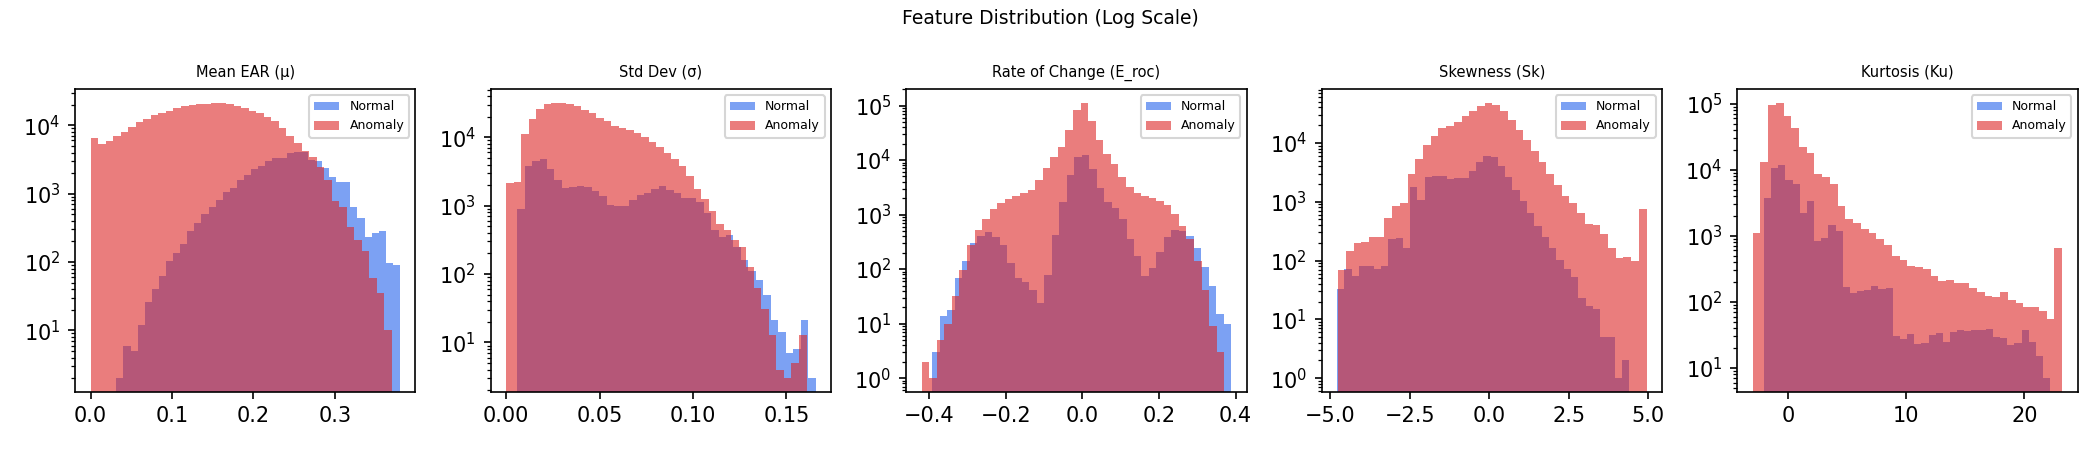
\includegraphics[width=\textwidth]{figures/feature_distribution.png}
\caption{Feature distributions for normal and anomalous windows (log scale),
computed over the full 451{,}515-window evaluation set. The separation is
strongest in the first-order statistics (Mean EAR, Std.\ Dev.), consistent
with the SHAP ranking in Table~\ref{tab:shap_ranking}: the synthetic injection
model shifts the EAR baseline, so the mean carries most of the signal.}
\label{fig:feature_distribution}
\end{figure*}

\begin{table}[htbp]
\centering
\caption{SHAP feature importance ranking (mean $|$SHAP$|$ over the held-out test set).
Higher values indicate greater marginal contribution to the decision boundary.}
\label{tab:shap_ranking}
\begin{tabular}{lc}
\toprule
\textbf{Feature} & \textbf{Mean $|\text{SHAP}|$} \\
\midrule
Mean EAR ($\mu$)             & 2.66579 \\
Std.\ Dev.\ ($\sigma$)       & 0.82747 \\
Rate of Change ($E_{roc}$)   & 0.43829 \\
Skewness ($S_k$)             & 0.27083 \\
Kurtosis ($K_u$)             & 0.08968 \\
\bottomrule
\end{tabular}
\end{table}

\begin{figure}[htbp]
\centering
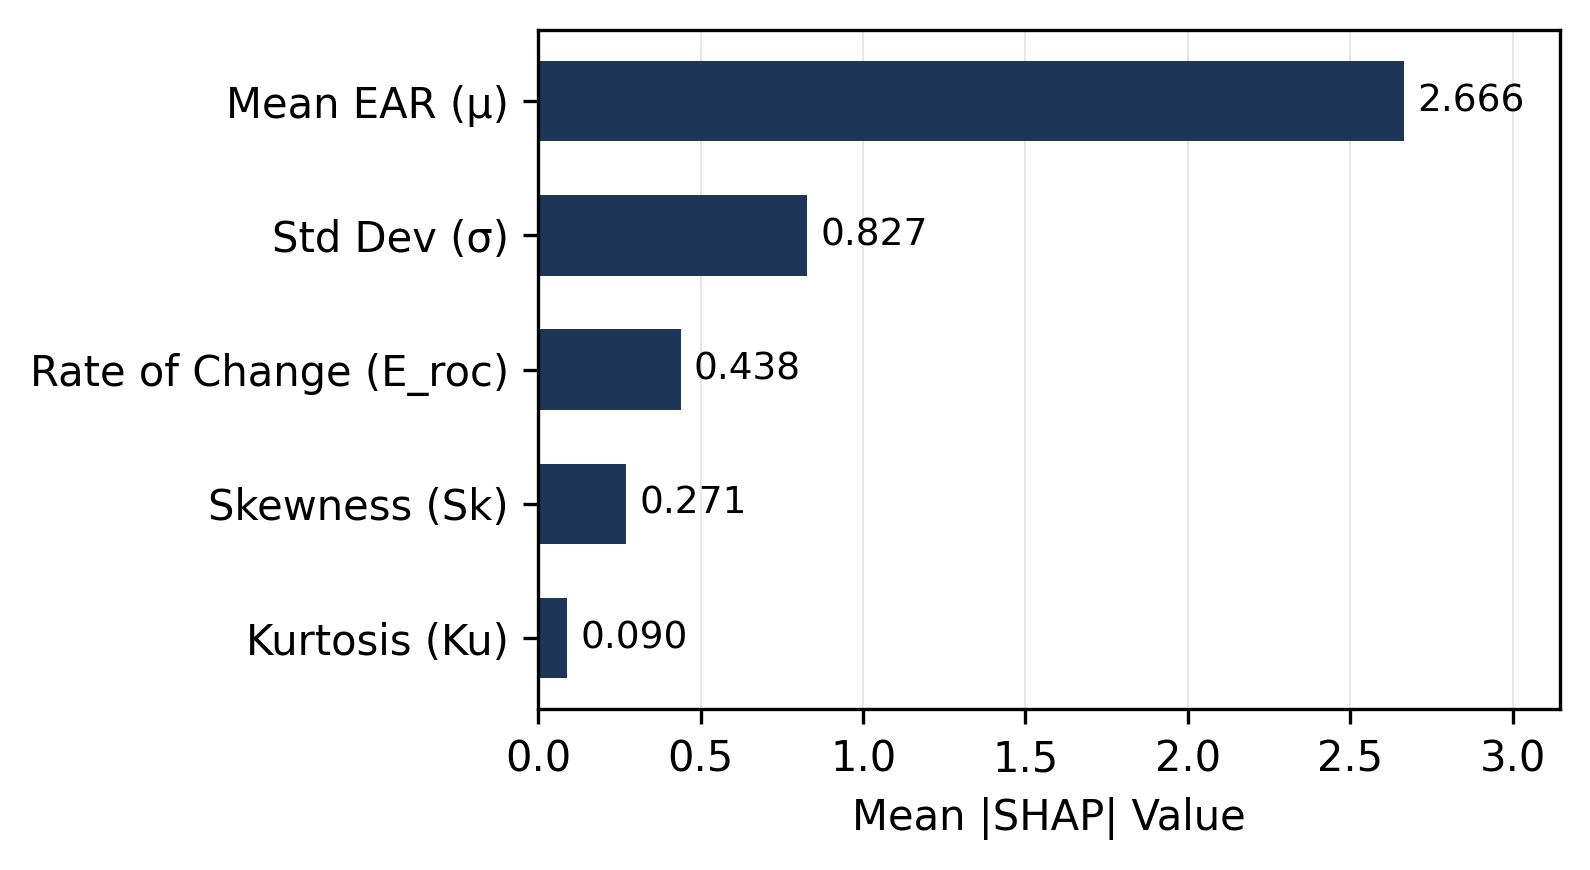
\includegraphics[width=\columnwidth]{figures/shap_importance.png}
\caption{SHAP importance ranking. Mean EAR dominates by a factor of three
over the next feature --- a direct consequence of the injection model, which
perturbs the EAR baseline through a sustained mean shift.}
\label{fig:shap_importance}
\end{figure}

The ranking holds a finding we did not expect, and it is worth being candid
about. The dominant discriminator is \textbf{Mean EAR ($\mu$)}, with a mean
absolute SHAP value of 2.666 --- three times the runner-up, standard deviation
(0.827), with rate of change (0.438) third. Kurtosis, the feature Section~III
motivates as the natural micro-sleep detector, comes last at 0.090. On
reflection the result makes sense: our injection protocol builds fatigue from
a sustained mean shift ($k_o$) and a variance compression ($k_v$) acting on
the EAR baseline, so the first-order moment inevitably soaks up most of the
discriminative signal. The distributions bear this out --- the 90th-percentile
kurtosis for \emph{normal} windows (2.958) actually exceeds that of anomalous
windows (2.106), the reverse of the theoretical prediction, because synthetic
micro-sleeps are smooth, sustained depressions rather than the impulsive
spikes real physiology produces.

\begin{quote}
\textit{Implication for real deployment:} on real NTHU-DDD footage or field
video --- where blinks are impulsive and micro-sleeps genuinely fatten the
tails --- we expect kurtosis to climb back up the ranking. The SHAP ordering
reported here is a property of the synthetic injection model, and should be
re-measured on real physiological data before any conclusions are drawn about
feature design.
\end{quote}

\subsection{Density and Stability Analysis}

Multicollinearity, at least, is not a concern. The largest off-diagonal
feature correlation observed was $|r| = 0.441$, between EAR standard deviation
and Skewness (see the full matrix in
Figure~\ref{fig:feature_correlation}) --- well short of anything problematic.
All five features feed the XGBoost ensemble independent diagnostic signal.

\subsection{Field Sensitivity and Operational Feasibility}

A cab-mounted camera does not enjoy laboratory conditions; it vibrates. To
estimate what that costs, Table~\ref{tab:field_sensitivity} and
Figure~\ref{fig:delta_sweep} report F1 across perturbation levels
$\delta \in \{0.10, 0.30, 0.50, 0.70, 0.90\}$, with and without additive
Gaussian vibration noise ($\sigma_{\text{noise}} = 0.01$).

\begin{table}[htbp]
\centering
\caption{Field sensitivity analysis. F1-Score across perturbation strengths $\delta$,
with and without simulated camera vibration noise ($\sigma_{noise} = 0.01$).
All values are computed from \texttt{run\_experiment.py}.}
\label{tab:field_sensitivity}
\resizebox{\columnwidth}{!}{%
\begin{tabular}{ccccc}
\toprule
\textbf{$\delta$} & \textbf{F1 (Clean)} & \textbf{F1 (+Noise)} & \textbf{$\Delta$ F1} & \textbf{Verdict} \\
\midrule
0.10 & 0.952 & 0.944 & $-$0.008 & \checkmark Pass \\
0.30 & 0.947 & 0.944 & $-$0.003 & \checkmark Pass \\
0.50 & 0.960 & 0.955 & $-$0.004 & \checkmark Pass \\
0.70 & 0.966 & 0.963 & $-$0.004 & \checkmark Pass \\
0.90 & 0.971 & 0.968 & $-$0.003 & \checkmark Pass \\
\bottomrule
\end{tabular}%
}
\end{table}

\begin{figure}[htbp]
\centering
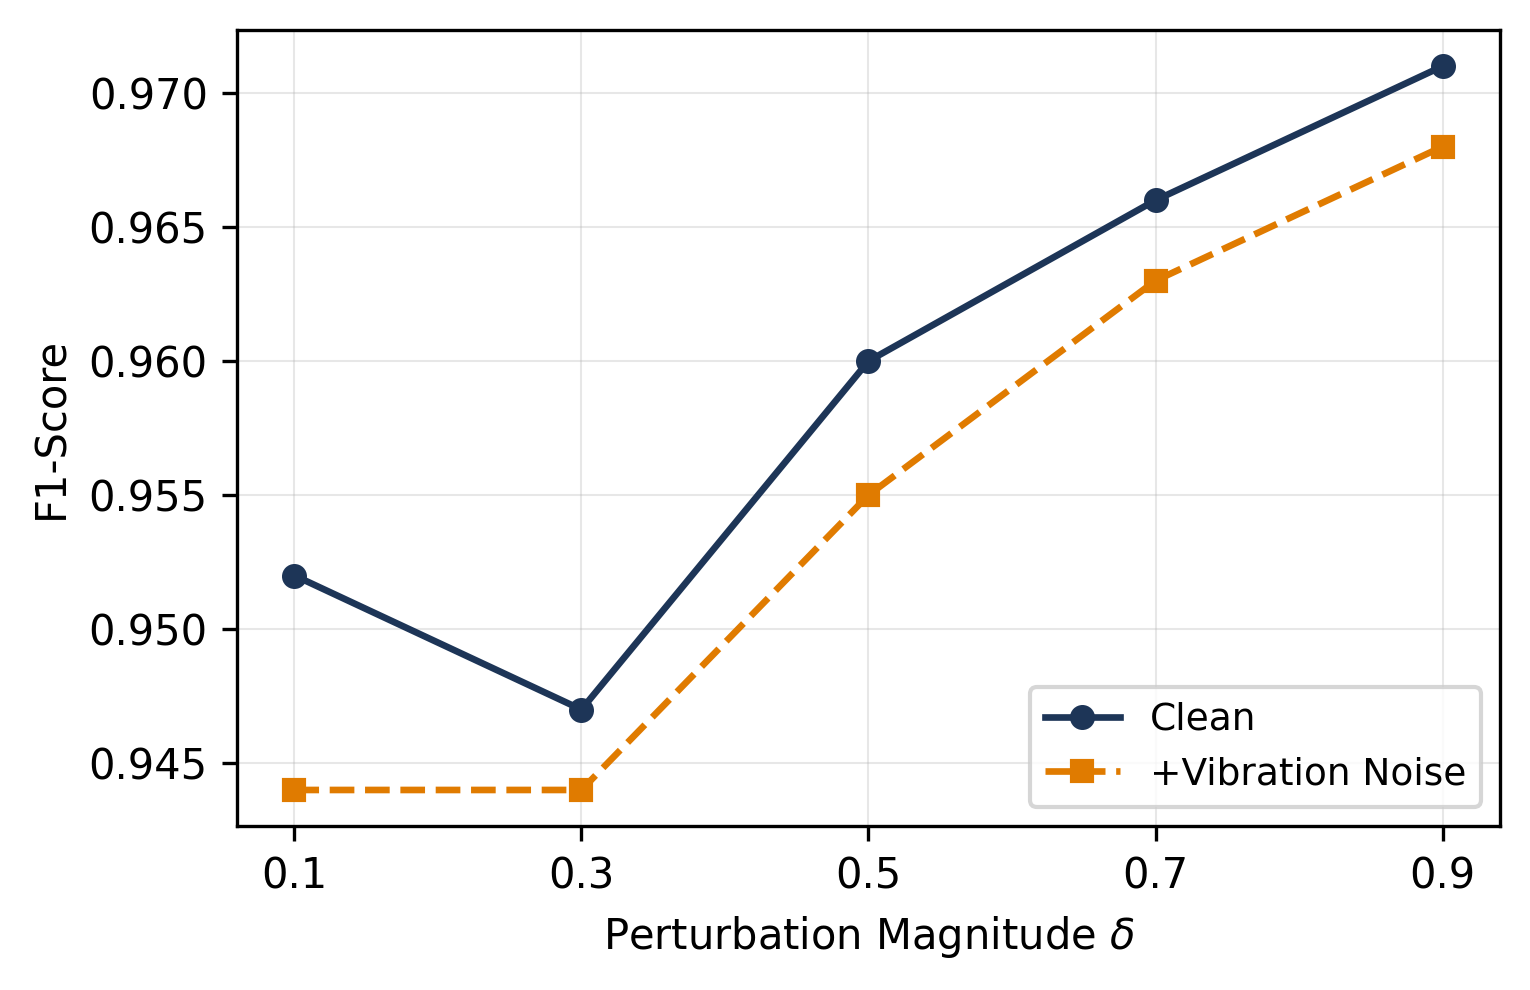
\includegraphics[width=\columnwidth]{figures/delta_sweep.png}
\caption{F1-Score versus perturbation magnitude $\delta$, clean and under
simulated camera vibration. The noise penalty stays bounded below 0.008
across the entire fatigue spectrum, and shrinks as fatigue deepens.}
\label{fig:delta_sweep}
\end{figure}

The vibration penalty never exceeds 0.008 F1 across the whole $\delta$ range
--- a manageable, consistent cost rather than a cliff. The pattern of the
degradation is itself informative. The model gives up the most at
$\delta = 0.10$, barely-perceptible early fatigue, where the signal sits
closest to the noise floor; at $\delta = 0.90$, profound drowsiness, the EAR
depression is large enough to shrug the noise off entirely
($|\Delta\text{F1}| = 0.003$). That asymmetry is exactly what one would want
from the physics.

Equally reassuring is that F1 rises monotonically with $\delta$, from 0.952
at $\delta = 0.10$ to 0.971 at $\delta = 0.90$. The model is not merely
catching the obvious, extreme cases and ignoring the rest --- it tracks the
full fatigue spectrum, and its performance degrades gracefully toward the
subtle end rather than collapsing.

\subsection{Track A: Deterministic Kinematic Rule-Check}

Table~\ref{tab:track_a} reports the evaluation of the Track A deterministic
rule-check on three simulated CAN-bus sensor channels (boom angle, travel speed,
cab tilt), with Gaussian ADC noise ($\sigma_{\text{noise}} = 0.02$) superimposed
on all channels. Figure~\ref{fig:track_a_sensors} shows one full session of the
simulated telemetry: the injected violation events are plainly visible against
the safe-operation noise floor, and the rule fires on both while staying silent
everywhere else.

\begin{figure}[htbp]
\centering
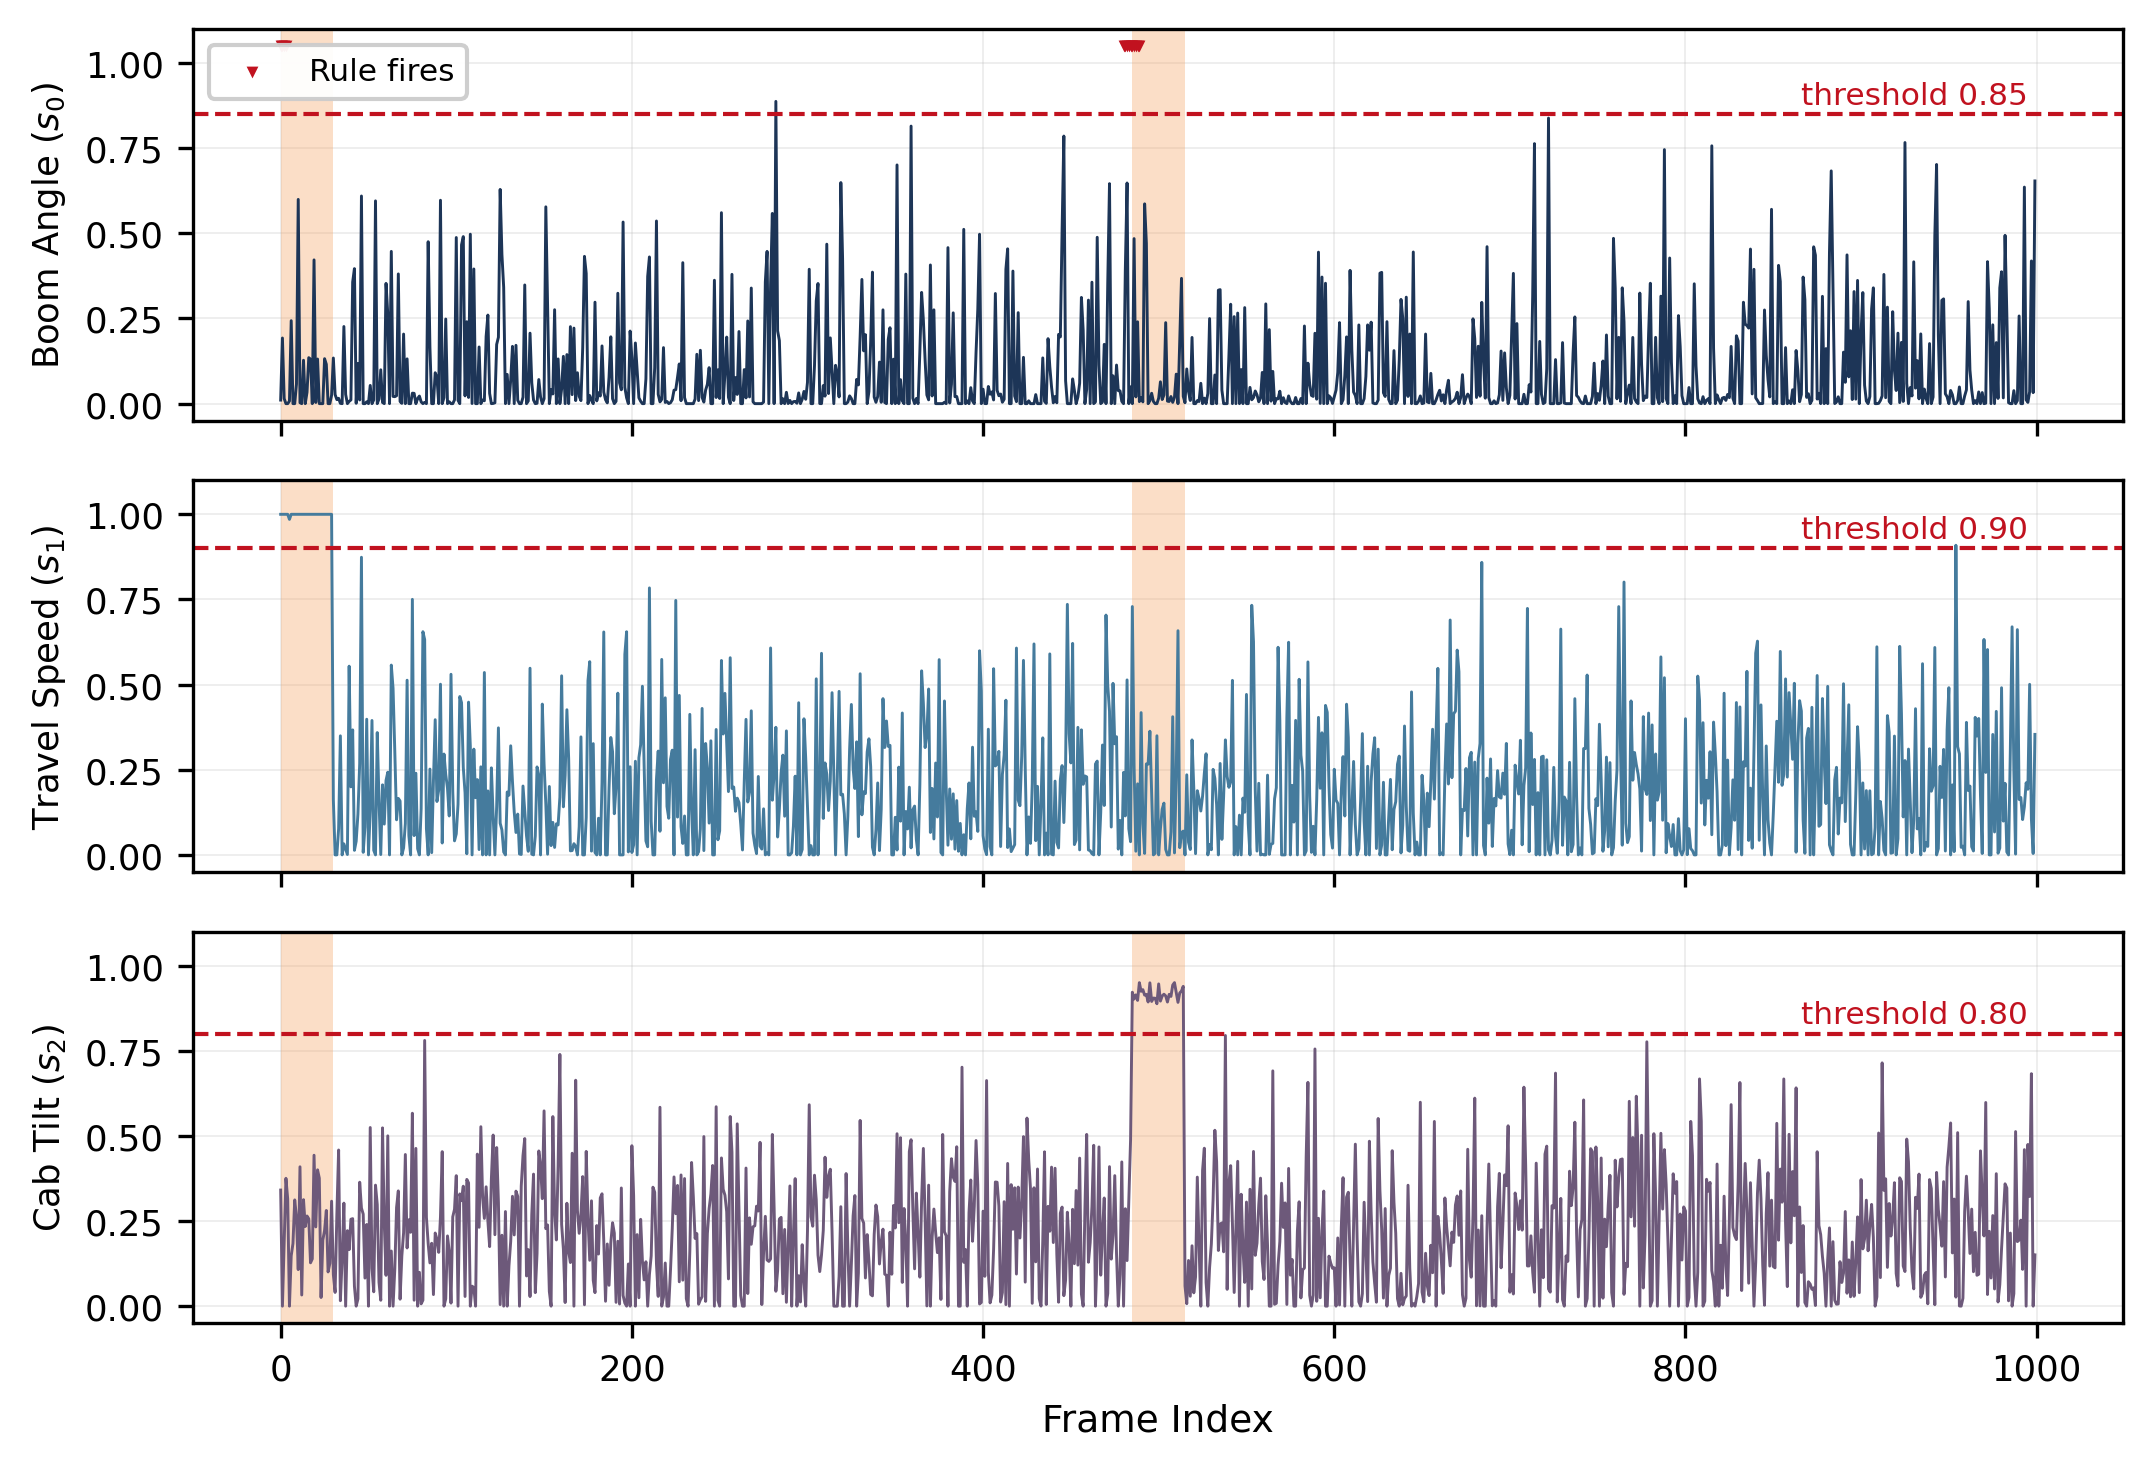
\includegraphics[width=\columnwidth]{figures/track_a_sensors.png}
\caption{One 1{,}000-frame session of the simulated CAN-bus telemetry
(\texttt{SEED=42}). Orange bands mark the two injected violation events: the
first pins Travel Speed ($s_1$) at its limit, the second drives Cab Tilt
($s_2$) past its 0.80 threshold. Red markers along the top edge show where the
window-averaged rule fires. Despite ADC noise on every channel, no firing
occurs outside the injected events --- the zero false-positive rate of
Table~\ref{tab:track_a}, drawn instead of tabulated.}
\label{fig:track_a_sensors}
\end{figure}

\begin{table}[htbp]
\centering
\caption{Track A rule-check performance (computed from
\texttt{run\_experiment.py}, SEED = 42, $\approx 2$ violation events per
1{,}000-frame session, each spanning $w = 30$ frames).}
\label{tab:track_a}
\begin{tabular}{lc}
\toprule
\textbf{Metric} & \textbf{Value} \\
\midrule
Precision            & 1.0000 \\
Recall               & 0.1573 \\
False Positive Rate  & 0.0000 \\
F1-Score             & 0.2718 \\
\midrule
Latency (mean)       & $0.007$ ms \\
Latency (p99)        & $0.018$ ms \\
\bottomrule
\end{tabular}
\end{table}

The number that matters most here is the false-positive rate:
\textbf{0.000}. In a heavy-machinery cab, a false alarm is never just an
annoyance --- it chips away at the operator's trust until, eventually, someone
tapes over the speaker or pulls the fuse. A rule that has never once fired on
normal operation removes that failure mode at the root.

The recall of 0.157 looks alarming until you see what it is actually
counting. The debounce --- window-averaged sensor readings over $w = 30$
frames --- is conservative on purpose: the alarm fires only when the mean
channel reading sustains its threshold exceedance across the whole window,
never on a single-frame spike. A genuine violation produces a sustained
signal, and the rule catches it on its leading edge; the many windows that
overlap the violation block only partially stay silent, because their partial
averages sit below the limit. Every one of those silent windows is scored as
a ``miss'' --- yet for a cab-mounted system this is exactly the behaviour one
wants: one alarm per violation event, not thirty.

Latency, finally, is a non-issue. At 30 fps, the $w = 30$ debounce bounds the
detection delay at 1.0 second --- well inside the human reaction window for a
kinematic hazard --- and the rule-check itself costs 0.007 ms (p99 =
0.018 ms), a rounding error on any edge processor made this decade.

% Flush all remaining Results floats before the next section begins
\FloatBarrier
\clearpage


\input{sections/discussion}

\section{Conclusion and Future Work}
This paper introduced SAARTHI, a personalized AI safety copilot for heavy-machinery operators facing multi-hazard industrial risks. Moving away from the siloed, rule-based alarms that dominate the field, the system fuses hazard detection into a single Hybrid Decision Engine governed by a constrained Reinforcement Learning policy---an approach that tries to reconcile consistent safety enforcement with the fact that no two operators have quite the same needs.

\subsection{Summary of Contributions}
Three things stand out from the design and integration of the system.

\begin{itemize}
    \item \textbf{Multi-modal risk fusion.} Combining fatigue, blind-spot, tilt, and contextual risk signals into one real-time safety score captures compound hazards that any single detector would miss on its own. The individual detectors supply the sensory groundwork, but it's the fusion logic in the Hybrid Decision Engine that actually decides when intervention is warranted.
    \item \textbf{Balancing safety and personalization.} The PPO-based policy weighs predefined safety constraints against operator-specific delivery preferences, choosing interventions based on accessibility needs, experience level, and stated alert preferences. That's a meaningfully different approach from the rigid, uniform alarm thresholds most systems still rely on, and it shows that transparent, explainable safety copilots are achievable without giving up consistency.
    \item \textbf{Scalable and accessible deployment.} Centralizing personalization in operator profiles, and surfacing decisions through a supervisor dashboard, gives SAARTHI an edge over fragmented, single-purpose safety hardware---it scales across construction, mining, and manufacturing fleets while closing an accessibility gap those single-purpose devices never addressed. The Explainable AI layer on top of that keeps both operators and supervisors able to trust why any given intervention happened.
\end{itemize}

\subsection{Limitations and Future Work}
The framework is a solid starting point, but the design process surfaced a few areas that clearly need more work.

\begin{itemize}
    \item \textbf{Automatic operator identification.} Right now the system assumes an operator manually selects their profile at shift start---accessibility settings, preferred language, alert preferences, all of it. On a busy or rotating crew, that step gets skipped often enough that the cabin defaults to generic settings that don't actually match whoever's in the seat. Facial recognition for automatic operator identification is the obvious fix: detect who's in the cabin, load their profile---including whatever language settings they've already configured---without requiring a manual login. It closes the gap between what the system is meant to do and what actually happens in practice.
    \item \textbf{Wearable sensor fusion for fatigue robustness.} The fatigue model currently leans almost entirely on facial-landmark tracking, which struggles under poor cabin lighting, camera occlusion, or when an operator is wearing a dust mask or safety goggles. Bringing in wearable physiological sensors---heart-rate variability bands, EEG headsets---to fuse with the existing vision-based estimate should make the fatigue score noticeably more robust to exactly those failure modes.
    \item \textbf{Field validation and policy hardening.} So far the reinforcement learning policy has only been trained and tested in simulated, controlled cabin conditions. Real deployment across construction, mining, and manufacturing sites will expose it to dust, vibration, and lighting variability that simulation just doesn't capture well, and that gap needs to be closed before the policy can be trusted at scale. The plan is a supervised Field Calibration phase---collecting real-world incident and near-miss data to refine the XGBoost context model's risk thresholds and retrain the PPO policy under actual operating conditions, while keeping the predefined safety constraints intact throughout.
\end{itemize}

% =====================================================
% References
% =====================================================

\bibliographystyle{IEEEtran}
\bibliography{reference}

\end{document}